\documentclass[1p]{elsarticle_modified}
%\bibliographystyle{elsarticle-num}

%\usepackage[colorlinks]{hyperref}
%\usepackage{abbrmath_seonhwa} %\Abb, \Ascr, \Acal ,\Abf, \Afrak
\usepackage{amsfonts}
\usepackage{amssymb}
\usepackage{amsmath}
\usepackage{amsthm}
\usepackage{scalefnt}
\usepackage{amsbsy}
\usepackage{kotex}
\usepackage{caption}
\usepackage{subfig}
\usepackage{color}
\usepackage{graphicx}
\usepackage{xcolor} %% white, black, red, green, blue, cyan, magenta, yellow
\usepackage{float}
\usepackage{setspace}
\usepackage{hyperref}

\usepackage{tikz}
\usetikzlibrary{arrows}

\usepackage{multirow}
\usepackage{array} % fixed length table
\usepackage{hhline}

%%%%%%%%%%%%%%%%%%%%%
\makeatletter
\renewcommand*\env@matrix[1][\arraystretch]{%
	\edef\arraystretch{#1}%
	\hskip -\arraycolsep
	\let\@ifnextchar\new@ifnextchar
	\array{*\c@MaxMatrixCols c}}
\makeatother %https://tex.stackexchange.com/questions/14071/how-can-i-increase-the-line-spacing-in-a-matrix
%%%%%%%%%%%%%%%

\usepackage[normalem]{ulem}

\newcommand{\msout}[1]{\ifmmode\text{\sout{\ensuremath{#1}}}\else\sout{#1}\fi}
%SOURCE: \msout is \stkout macro in https://tex.stackexchange.com/questions/20609/strikeout-in-math-mode

\newcommand{\cancel}[1]{
	\ifmmode
	{\color{red}\msout{#1}}
	\else
	{\color{red}\sout{#1}}
	\fi
}

\newcommand{\add}[1]{
	{\color{blue}\uwave{#1}}
}

\newcommand{\replace}[2]{
	\ifmmode
	{\color{red}\msout{#1}}{\color{blue}\uwave{#2}}
	\else
	{\color{red}\sout{#1}}{\color{blue}\uwave{#2}}
	\fi
}

\newcommand{\Sol}{\mathcal{S}} %segment
\newcommand{\D}{D} %diagram
\newcommand{\A}{\mathcal{A}} %arc


%%%%%%%%%%%%%%%%%%%%%%%%%%%%%5 test

\def\sl{\operatorname{\textup{SL}}(2,\Cbb)}
\def\psl{\operatorname{\textup{PSL}}(2,\Cbb)}
\def\quan{\mkern 1mu \triangleright \mkern 1mu}

\theoremstyle{definition}
\newtheorem{thm}{Theorem}[section]
\newtheorem{prop}[thm]{Proposition}
\newtheorem{lem}[thm]{Lemma}
\newtheorem{ques}[thm]{Question}
\newtheorem{cor}[thm]{Corollary}
\newtheorem{defn}[thm]{Definition}
\newtheorem{exam}[thm]{Example}
\newtheorem{rmk}[thm]{Remark}
\newtheorem{alg}[thm]{Algorithm}

\newcommand{\I}{\sqrt{-1}}
\begin{document}

%\begin{frontmatter}
%
%\title{Boundary parabolic representations of knots up to 8 crossings}
%
%%% Group authors per affiliation:
%\author{Yunhi Cho} 
%\address{Department of Mathematics, University of Seoul, Seoul, Korea}
%\ead{yhcho@uos.ac.kr}
%
%
%\author{Seonhwa Kim} %\fnref{s_kim}}
%\address{Center for Geometry and Physics, Institute for Basic Science, Pohang, 37673, Korea}
%\ead{ryeona17@ibs.re.kr}
%
%\author{Hyuk Kim}
%\address{Department of Mathematical Sciences, Seoul National University, Seoul 08826, Korea}
%\ead{hyukkim@snu.ac.kr}
%
%\author{Seokbeom Yoon}
%\address{Department of Mathematical Sciences, Seoul National University, Seoul, 08826,  Korea}
%\ead{sbyoon15@snu.ac.kr}
%
%\begin{abstract}
%We find all boundary parabolic representation of knots up to 8 crossings.
%
%\end{abstract}
%\begin{keyword}
%    \MSC[2010] 57M25 
%\end{keyword}
%
%\end{frontmatter}

%\linenumbers
%\tableofcontents
%
\newcommand\colored[1]{\textcolor{white}{\rule[-0.35ex]{0.8em}{1.4ex}}\kern-0.8em\color{red} #1}%
%\newcommand\colored[1]{\textcolor{white}{ #1}\kern-2.17ex	\textcolor{white}{ #1}\kern-1.81ex	\textcolor{white}{ #1}\kern-2.15ex\color{red}#1	}

{\Large $\underline{12a_{0360}~(K12a_{0360})}$}

\setlength{\tabcolsep}{10pt}
\renewcommand{\arraystretch}{1.6}
\vspace{1cm}\begin{tabular}{m{100pt}>{\centering\arraybackslash}m{274pt}}
\multirow{5}{120pt}{
	\centering
	\includegraphics[width=112pt]{../../../GIT/diagram.site/Diagrams/png/1161_12a_0360.png}\\
\ \ \ A knot diagram\footnotemark}&
\allowdisplaybreaks
\textbf{Linearized knot diagam} \\
\cline{2-2}
 &
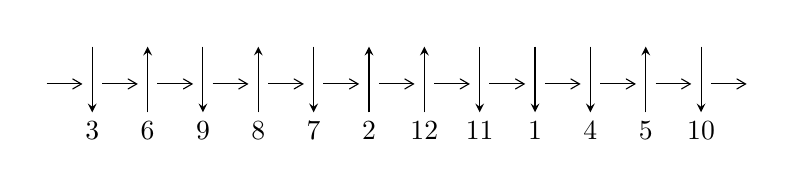
\begin{tikzpicture}[x=20pt, y=17pt]
	% nodes
	\node (C0) at (0, 0) {};
	\node (C1) at (1, 0) {};
	\node (C1U) at (1, +1) {};
	\node (C1D) at (1, -1) {3};

	\node (C2) at (2, 0) {};
	\node (C2U) at (2, +1) {};
	\node (C2D) at (2, -1) {6};

	\node (C3) at (3, 0) {};
	\node (C3U) at (3, +1) {};
	\node (C3D) at (3, -1) {9};

	\node (C4) at (4, 0) {};
	\node (C4U) at (4, +1) {};
	\node (C4D) at (4, -1) {8};

	\node (C5) at (5, 0) {};
	\node (C5U) at (5, +1) {};
	\node (C5D) at (5, -1) {7};

	\node (C6) at (6, 0) {};
	\node (C6U) at (6, +1) {};
	\node (C6D) at (6, -1) {2};

	\node (C7) at (7, 0) {};
	\node (C7U) at (7, +1) {};
	\node (C7D) at (7, -1) {12};

	\node (C8) at (8, 0) {};
	\node (C8U) at (8, +1) {};
	\node (C8D) at (8, -1) {11};

	\node (C9) at (9, 0) {};
	\node (C9U) at (9, +1) {};
	\node (C9D) at (9, -1) {1};

	\node (C10) at (10, 0) {};
	\node (C10U) at (10, +1) {};
	\node (C10D) at (10, -1) {4};

	\node (C11) at (11, 0) {};
	\node (C11U) at (11, +1) {};
	\node (C11D) at (11, -1) {5};

	\node (C12) at (12, 0) {};
	\node (C12U) at (12, +1) {};
	\node (C12D) at (12, -1) {10};
	\node (C13) at (13, 0) {};

	% arrows
	\draw[->,>={angle 60}]
	(C0) edge (C1) (C1) edge (C2) (C2) edge (C3) (C3) edge (C4) (C4) edge (C5) (C5) edge (C6) (C6) edge (C7) (C7) edge (C8) (C8) edge (C9) (C9) edge (C10) (C10) edge (C11) (C11) edge (C12) (C12) edge (C13) ;	\draw[->,>=stealth]
	(C1U) edge (C1D) (C2D) edge (C2U) (C3U) edge (C3D) (C4D) edge (C4U) (C5U) edge (C5D) (C6D) edge (C6U) (C7D) edge (C7U) (C8U) edge (C8D) (C9U) edge (C9D) (C10U) edge (C10D) (C11D) edge (C11U) (C12U) edge (C12D) ;
	\end{tikzpicture} \\
\hhline{~~} \\& 
\textbf{Solving Sequence} \\ \cline{2-2} 
 &
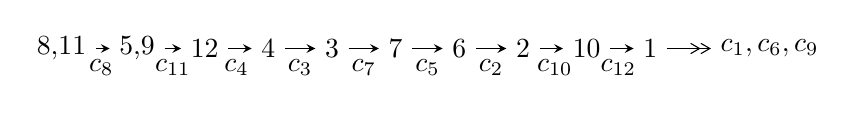
\begin{tikzpicture}[x=23pt, y=7pt]
	% node
	\node (A0) at (-1/8, 0) {8,11};
	\node (A1) at (17/16, 0) {5,9};
	\node (A2) at (17/8, 0) {12};
	\node (A3) at (25/8, 0) {4};
	\node (A4) at (33/8, 0) {3};
	\node (A5) at (41/8, 0) {7};
	\node (A6) at (49/8, 0) {6};
	\node (A7) at (57/8, 0) {2};
	\node (A8) at (65/8, 0) {10};
	\node (A9) at (73/8, 0) {1};
	\node (C1) at (1/2, -1) {$c_{8}$};
	\node (C2) at (13/8, -1) {$c_{11}$};
	\node (C3) at (21/8, -1) {$c_{4}$};
	\node (C4) at (29/8, -1) {$c_{3}$};
	\node (C5) at (37/8, -1) {$c_{7}$};
	\node (C6) at (45/8, -1) {$c_{5}$};
	\node (C7) at (53/8, -1) {$c_{2}$};
	\node (C8) at (61/8, -1) {$c_{10}$};
	\node (C9) at (69/8, -1) {$c_{12}$};
	\node (A10) at (11, 0) {$c_{1},c_{6},c_{9}$};

	% edge
	\draw[->,>=stealth]	
	(A0) edge (A1) (A1) edge (A2) (A2) edge (A3) (A3) edge (A4) (A4) edge (A5) (A5) edge (A6) (A6) edge (A7) (A7) edge (A8) (A8) edge (A9) ;
	\draw[->>,>={angle 60}]	
	(A9) edge (A10);
\end{tikzpicture} \\ 

\end{tabular} \\

\footnotetext{
The image of knot diagram is generated by the software ``\textbf{Draw programme}" developed by Andrew Bartholomew(\url{http://www.layer8.co.uk/maths/draw/index.htm\#Running-draw}), where we modified some parts for our purpose(\url{https://github.com/CATsTAILs/LinksPainter}).
}\phantom \\ \newline 
\centering \textbf{Ideals for irreducible components\footnotemark of $X_{\text{par}}$} 
 
\begin{align*}
I^u_{1}&=\langle 
-3.30570\times10^{1105} u^{145}-4.41286\times10^{1106} u^{144}+\cdots+1.33638\times10^{1108} b-8.24729\times10^{1108},\\
\phantom{I^u_{1}}&\phantom{= \langle  }-6.53292\times10^{1106} u^{145}-8.61380\times10^{1107} u^{144}+\cdots+5.34553\times10^{1108} a-1.10086\times10^{1110},\\
\phantom{I^u_{1}}&\phantom{= \langle  }u^{146}+13 u^{145}+\cdots+3712 u+768\rangle \\
I^u_{2}&=\langle 
7.17507\times10^{32} u^{25}-3.74911\times10^{33} u^{24}+\cdots+2.20341\times10^{33} b-2.57469\times10^{35},\\
\phantom{I^u_{2}}&\phantom{= \langle  }7.48722\times10^{34} u^{25}-3.83632\times10^{35} u^{24}+\cdots+1.43222\times10^{35} a-2.61037\times10^{37},\\
\phantom{I^u_{2}}&\phantom{= \langle  }u^{26}-6 u^{25}+\cdots-1450 u+325\rangle \\
\\
I^v_{1}&=\langle 
a,\;- v^2+b+2 v,\;v^4-3 v^3+2 v^2+1\rangle \\
I^v_{2}&=\langle 
a,\;-5 v^3+16 v^2+8 b-40 v+15,\;v^4-3 v^3+8 v^2-3 v+1\rangle \\
\end{align*}
\raggedright * 4 irreducible components of $\dim_{\mathbb{C}}=0$, with total 180 representations.\\
\footnotetext{All coefficients of polynomials are rational numbers. But the coefficients are sometimes approximated in decimal forms when there is not enough margin.}
\newpage
\renewcommand{\arraystretch}{1}
\centering \section*{I. $I^u_{1}= \langle -3.31\times10^{1105} u^{145}-4.41\times10^{1106} u^{144}+\cdots+1.34\times10^{1108} b-8.25\times10^{1108},\;-6.53\times10^{1106} u^{145}-8.61\times10^{1107} u^{144}+\cdots+5.35\times10^{1108} a-1.10\times10^{1110},\;u^{146}+13 u^{145}+\cdots+3712 u+768 \rangle$}
\flushleft \textbf{(i) Arc colorings}\\
\begin{tabular}{m{7pt} m{180pt} m{7pt} m{180pt} }
\flushright $a_{8}=$&$\begin{pmatrix}1\\0\end{pmatrix}$ \\
\flushright $a_{11}=$&$\begin{pmatrix}0\\u\end{pmatrix}$ \\
\flushright $a_{5}=$&$\begin{pmatrix}0.0122213 u^{145}+0.161140 u^{144}+\cdots+123.861 u+20.5939\\0.00247362 u^{145}+0.0330209 u^{144}+\cdots+31.3706 u+6.17135\end{pmatrix}$ \\
\flushright $a_{9}=$&$\begin{pmatrix}1\\u^2\end{pmatrix}$ \\
\flushright $a_{12}=$&$\begin{pmatrix}-0.00406636 u^{145}-0.0533296 u^{144}+\cdots-47.0455 u-7.79538\\-0.000663045 u^{145}-0.00907307 u^{144}+\cdots-11.0244 u-2.37289\end{pmatrix}$ \\
\flushright $a_{4}=$&$\begin{pmatrix}0.00974766 u^{145}+0.128119 u^{144}+\cdots+92.4900 u+14.4226\\0.00247362 u^{145}+0.0330209 u^{144}+\cdots+31.3706 u+6.17135\end{pmatrix}$ \\
\flushright $a_{3}=$&$\begin{pmatrix}0.0143319 u^{145}+0.188459 u^{144}+\cdots+136.542 u+21.6688\\0.00140153 u^{145}+0.0192365 u^{144}+\cdots+25.0843 u+5.59915\end{pmatrix}$ \\
\flushright $a_{7}=$&$\begin{pmatrix}0.00508132 u^{145}+0.0632419 u^{144}+\cdots+9.88946 u-3.18855\\0.000960881 u^{145}+0.0115579 u^{144}+\cdots+3.55703 u-0.539101\end{pmatrix}$ \\
\flushright $a_{6}=$&$\begin{pmatrix}-0.0202071 u^{145}-0.269862 u^{144}+\cdots-246.988 u-42.3344\\-0.000188244 u^{145}-0.00491796 u^{144}+\cdots-44.8135 u-10.4290\end{pmatrix}$ \\
\flushright $a_{2}=$&$\begin{pmatrix}-0.00444409 u^{145}-0.0545649 u^{144}+\cdots-3.69753 u+4.61182\\-0.000951740 u^{145}-0.0118936 u^{144}+\cdots-7.64145 u-0.530581\end{pmatrix}$ \\
\flushright $a_{10}=$&$\begin{pmatrix}-0.00366625 u^{145}-0.0476731 u^{144}+\cdots-30.5632 u-4.50047\\0.000262933 u^{145}+0.00341664 u^{144}+\cdots-3.45791 u-0.922013\end{pmatrix}$ \\
\flushright $a_{1}=$&$\begin{pmatrix}-0.00241677 u^{145}-0.0308188 u^{144}+\cdots-10.6699 u-0.449860\\-0.000892350 u^{145}-0.0114009 u^{144}+\cdots-5.71646 u-0.449654\end{pmatrix}$\\&\end{tabular}
\flushleft \textbf{(ii) Obstruction class $= -1$}\\~\\
\flushleft \textbf{(iii) Cusp Shapes $= -0.00659825 u^{145}-0.0907768 u^{144}+\cdots-143.657 u-31.5748$}\\~\\
\newpage\renewcommand{\arraystretch}{1}
\flushleft \textbf{(iv) u-Polynomials at the component}\newline \\
\begin{tabular}{m{50pt}|m{274pt}}
Crossings & \hspace{64pt}u-Polynomials at each crossing \\
\hline $$\begin{aligned}c_{1},c_{5}\end{aligned}$$&$\begin{aligned}
&u^{146}+41 u^{145}+\cdots+13874 u+441
\end{aligned}$\\
\hline $$\begin{aligned}c_{2},c_{6}\end{aligned}$$&$\begin{aligned}
&u^{146}-3 u^{145}+\cdots+56 u+21
\end{aligned}$\\
\hline $$\begin{aligned}c_{3}\end{aligned}$$&$\begin{aligned}
&u^{146}+3 u^{145}+\cdots-213878079 u+69993509
\end{aligned}$\\
\hline $$\begin{aligned}c_{4}\end{aligned}$$&$\begin{aligned}
&u^{146}+9 u^{145}+\cdots+97 u+16
\end{aligned}$\\
\hline $$\begin{aligned}c_{7}\end{aligned}$$&$\begin{aligned}
&u^{146}-5 u^{145}+\cdots+163744 u+32887
\end{aligned}$\\
\hline $$\begin{aligned}c_{8}\end{aligned}$$&$\begin{aligned}
&u^{146}-13 u^{145}+\cdots-3712 u+768
\end{aligned}$\\
\hline $$\begin{aligned}c_{9},c_{12}\end{aligned}$$&$\begin{aligned}
&u^{146}+7 u^{145}+\cdots+95533 u+4448
\end{aligned}$\\
\hline $$\begin{aligned}c_{10}\end{aligned}$$&$\begin{aligned}
&u^{146}-6 u^{144}+\cdots-35 u+1
\end{aligned}$\\
\hline $$\begin{aligned}c_{11}\end{aligned}$$&$\begin{aligned}
&u^{146}+2 u^{145}+\cdots+153777 u+21323
\end{aligned}$\\
\hline
\end{tabular}\\~\\
\newpage\renewcommand{\arraystretch}{1}
\flushleft \textbf{(v) Riley Polynomials at the component}\newline \\
\begin{tabular}{m{50pt}|m{274pt}}
Crossings & \hspace{64pt}Riley Polynomials at each crossing \\
\hline $$\begin{aligned}c_{1},c_{5}\end{aligned}$$&$\begin{aligned}
&y^{146}+141 y^{145}+\cdots+10798130 y+194481
\end{aligned}$\\
\hline $$\begin{aligned}c_{2},c_{6}\end{aligned}$$&$\begin{aligned}
&y^{146}+41 y^{145}+\cdots+13874 y+441
\end{aligned}$\\
\hline $$\begin{aligned}c_{3}\end{aligned}$$&$\begin{aligned}
&y^{146}+59 y^{145}+\cdots+839682611759848865 y+4899091302133081
\end{aligned}$\\
\hline $$\begin{aligned}c_{4}\end{aligned}$$&$\begin{aligned}
&y^{146}+21 y^{145}+\cdots+13375 y+256
\end{aligned}$\\
\hline $$\begin{aligned}c_{7}\end{aligned}$$&$\begin{aligned}
&y^{146}-39 y^{145}+\cdots-49681388466 y+1081554769
\end{aligned}$\\
\hline $$\begin{aligned}c_{8}\end{aligned}$$&$\begin{aligned}
&y^{146}+11 y^{145}+\cdots+6373376 y+589824
\end{aligned}$\\
\hline $$\begin{aligned}c_{9},c_{12}\end{aligned}$$&$\begin{aligned}
&y^{146}+97 y^{145}+\cdots-4451394729 y+19784704
\end{aligned}$\\
\hline $$\begin{aligned}c_{10}\end{aligned}$$&$\begin{aligned}
&y^{146}-12 y^{145}+\cdots+265 y+1
\end{aligned}$\\
\hline $$\begin{aligned}c_{11}\end{aligned}$$&$\begin{aligned}
&y^{146}-30 y^{145}+\cdots-28764118101 y+454670329
\end{aligned}$\\
\hline
\end{tabular}\\~\\
\newpage\flushleft \textbf{(vi) Complex Volumes and Cusp Shapes}
$$\begin{array}{c|c|c}  
\text{Solutions to }I^u_{1}& \I (\text{vol} + \sqrt{-1}CS) & \text{Cusp shape}\\
 \hline 
\begin{aligned}
u &= -0.802454 + 0.588037 I \\
a &= -0.531807 - 1.135870 I \\
b &= -1.020260 - 0.872880 I\end{aligned}
 & \phantom{-}3.29509 + 2.59410 I & \phantom{-0.000000 } 0 \\ \hline\begin{aligned}
u &= -0.802454 - 0.588037 I \\
a &= -0.531807 + 1.135870 I \\
b &= -1.020260 + 0.872880 I\end{aligned}
 & \phantom{-}3.29509 - 2.59410 I & \phantom{-0.000000 } 0 \\ \hline\begin{aligned}
u &= \phantom{-}0.871003 + 0.506893 I \\
a &= \phantom{-}0.403140 - 0.851076 I \\
b &= \phantom{-}1.20409 - 1.11526 I\end{aligned}
 & -1.65989 - 5.49131 I & \phantom{-0.000000 } 0 \\ \hline\begin{aligned}
u &= \phantom{-}0.871003 - 0.506893 I \\
a &= \phantom{-}0.403140 + 0.851076 I \\
b &= \phantom{-}1.20409 + 1.11526 I\end{aligned}
 & -1.65989 + 5.49131 I & \phantom{-0.000000 } 0 \\ \hline\begin{aligned}
u &= \phantom{-}0.429141 + 0.917197 I \\
a &= -0.201495 + 0.959077 I \\
b &= -0.87385 + 1.26504 I\end{aligned}
 & \phantom{-}1.51786 - 4.56864 I & \phantom{-0.000000 } 0 \\ \hline\begin{aligned}
u &= \phantom{-}0.429141 - 0.917197 I \\
a &= -0.201495 - 0.959077 I \\
b &= -0.87385 - 1.26504 I\end{aligned}
 & \phantom{-}1.51786 + 4.56864 I & \phantom{-0.000000 } 0 \\ \hline\begin{aligned}
u &= -0.827144 + 0.492973 I \\
a &= \phantom{-}0.616486 + 1.195440 I \\
b &= \phantom{-}1.07282 + 0.96391 I\end{aligned}
 & \phantom{-}2.42208 + 8.12198 I & \phantom{-0.000000 } 0 \\ \hline\begin{aligned}
u &= -0.827144 - 0.492973 I \\
a &= \phantom{-}0.616486 - 1.195440 I \\
b &= \phantom{-}1.07282 - 0.96391 I\end{aligned}
 & \phantom{-}2.42208 - 8.12198 I & \phantom{-0.000000 } 0 \\ \hline\begin{aligned}
u &= \phantom{-}0.748394 + 0.604038 I \\
a &= -0.598029 - 0.270701 I \\
b &= \phantom{-}0.205977 - 0.532694 I\end{aligned}
 & -1.38423 - 0.78057 I & \phantom{-0.000000 } 0 \\ \hline\begin{aligned}
u &= \phantom{-}0.748394 - 0.604038 I \\
a &= -0.598029 + 0.270701 I \\
b &= \phantom{-}0.205977 + 0.532694 I\end{aligned}
 & -1.38423 + 0.78057 I & \phantom{-0.000000 } 0\\
 \hline 
 \end{array}$$\newpage$$\begin{array}{c|c|c}  
\text{Solutions to }I^u_{1}& \I (\text{vol} + \sqrt{-1}CS) & \text{Cusp shape}\\
 \hline 
\begin{aligned}
u &= -0.508387 + 0.924849 I \\
a &= -0.960150 - 0.195445 I \\
b &= \phantom{-}0.387156 + 0.376888 I\end{aligned}
 & \phantom{-}3.13027 + 3.31987 I & \phantom{-0.000000 } 0 \\ \hline\begin{aligned}
u &= -0.508387 - 0.924849 I \\
a &= -0.960150 + 0.195445 I \\
b &= \phantom{-}0.387156 - 0.376888 I\end{aligned}
 & \phantom{-}3.13027 - 3.31987 I & \phantom{-0.000000 } 0 \\ \hline\begin{aligned}
u &= \phantom{-}0.053551 + 0.932125 I \\
a &= -0.161722 - 1.071830 I \\
b &= -1.021500 - 0.623407 I\end{aligned}
 & \phantom{-}6.30567 + 0.04181 I & \phantom{-0.000000 } 0 \\ \hline\begin{aligned}
u &= \phantom{-}0.053551 - 0.932125 I \\
a &= -0.161722 + 1.071830 I \\
b &= -1.021500 + 0.623407 I\end{aligned}
 & \phantom{-}6.30567 - 0.04181 I & \phantom{-0.000000 } 0 \\ \hline\begin{aligned}
u &= \phantom{-}0.137828 + 0.917504 I \\
a &= \phantom{-}0.168695 + 1.034250 I \\
b &= \phantom{-}1.060330 + 0.607548 I\end{aligned}
 & \phantom{-}5.81980 - 6.06300 I & \phantom{-0.000000 } 0 \\ \hline\begin{aligned}
u &= \phantom{-}0.137828 - 0.917504 I \\
a &= \phantom{-}0.168695 - 1.034250 I \\
b &= \phantom{-}1.060330 - 0.607548 I\end{aligned}
 & \phantom{-}5.81980 + 6.06300 I & \phantom{-0.000000 } 0 \\ \hline\begin{aligned}
u &= \phantom{-}1.078310 + 0.012960 I \\
a &= \phantom{-}0.48197 + 1.49587 I \\
b &= \phantom{-}0.065355 + 0.580528 I\end{aligned}
 & -3.69081 - 0.08768 I & \phantom{-0.000000 } 0 \\ \hline\begin{aligned}
u &= \phantom{-}1.078310 - 0.012960 I \\
a &= \phantom{-}0.48197 - 1.49587 I \\
b &= \phantom{-}0.065355 - 0.580528 I\end{aligned}
 & -3.69081 + 0.08768 I & \phantom{-0.000000 } 0 \\ \hline\begin{aligned}
u &= -0.961574 + 0.533261 I \\
a &= \phantom{-}1.22512 - 1.29575 I \\
b &= -0.332786 - 0.684088 I\end{aligned}
 & \phantom{-}6.09233 + 10.74490 I & \phantom{-0.000000 } 0 \\ \hline\begin{aligned}
u &= -0.961574 - 0.533261 I \\
a &= \phantom{-}1.22512 + 1.29575 I \\
b &= -0.332786 + 0.684088 I\end{aligned}
 & \phantom{-}6.09233 - 10.74490 I & \phantom{-0.000000 } 0\\
 \hline 
 \end{array}$$\newpage$$\begin{array}{c|c|c}  
\text{Solutions to }I^u_{1}& \I (\text{vol} + \sqrt{-1}CS) & \text{Cusp shape}\\
 \hline 
\begin{aligned}
u &= -1.082670 + 0.263362 I \\
a &= -0.663520 + 0.363145 I \\
b &= -0.287318 + 0.715534 I\end{aligned}
 & \phantom{-}1.32164 - 2.89842 I & \phantom{-0.000000 } 0 \\ \hline\begin{aligned}
u &= -1.082670 - 0.263362 I \\
a &= -0.663520 - 0.363145 I \\
b &= -0.287318 - 0.715534 I\end{aligned}
 & \phantom{-}1.32164 + 2.89842 I & \phantom{-0.000000 } 0 \\ \hline\begin{aligned}
u &= -0.224981 + 0.850372 I \\
a &= \phantom{-}0.344235 + 0.246836 I \\
b &= \phantom{-}0.471852 - 0.683778 I\end{aligned}
 & -1.85922 - 1.49457 I & \phantom{-0.000000 } 0 \\ \hline\begin{aligned}
u &= -0.224981 - 0.850372 I \\
a &= \phantom{-}0.344235 - 0.246836 I \\
b &= \phantom{-}0.471852 + 0.683778 I\end{aligned}
 & -1.85922 + 1.49457 I & \phantom{-0.000000 } 0 \\ \hline\begin{aligned}
u &= -0.969668 + 0.612996 I \\
a &= -1.10536 + 1.17499 I \\
b &= \phantom{-}0.373015 + 0.672914 I\end{aligned}
 & \phantom{-}6.68296 + 4.72439 I & \phantom{-0.000000 } 0 \\ \hline\begin{aligned}
u &= -0.969668 - 0.612996 I \\
a &= -1.10536 - 1.17499 I \\
b &= \phantom{-}0.373015 - 0.672914 I\end{aligned}
 & \phantom{-}6.68296 - 4.72439 I & \phantom{-0.000000 } 0 \\ \hline\begin{aligned}
u &= -0.560635 + 1.006060 I \\
a &= -0.335631 + 0.864108 I \\
b &= \phantom{-}1.19675 + 1.16993 I\end{aligned}
 & -1.13829 + 5.55339 I & \phantom{-0.000000 } 0 \\ \hline\begin{aligned}
u &= -0.560635 - 1.006060 I \\
a &= -0.335631 - 0.864108 I \\
b &= \phantom{-}1.19675 - 1.16993 I\end{aligned}
 & -1.13829 - 5.55339 I & \phantom{-0.000000 } 0 \\ \hline\begin{aligned}
u &= \phantom{-}0.092261 + 0.821801 I \\
a &= \phantom{-}0.88761 + 1.79345 I \\
b &= -0.980157 + 0.518850 I\end{aligned}
 & \phantom{-}11.02230 - 3.86586 I & \phantom{-0.000000 } 0 \\ \hline\begin{aligned}
u &= \phantom{-}0.092261 - 0.821801 I \\
a &= \phantom{-}0.88761 - 1.79345 I \\
b &= -0.980157 - 0.518850 I\end{aligned}
 & \phantom{-}11.02230 + 3.86586 I & \phantom{-0.000000 } 0\\
 \hline 
 \end{array}$$\newpage$$\begin{array}{c|c|c}  
\text{Solutions to }I^u_{1}& \I (\text{vol} + \sqrt{-1}CS) & \text{Cusp shape}\\
 \hline 
\begin{aligned}
u &= -0.617603 + 0.545779 I \\
a &= \phantom{-}1.97468 - 0.58063 I \\
b &= -0.263967 - 0.519798 I\end{aligned}
 & -0.28583 + 5.92748 I & \phantom{-0.000000 } 0 \\ \hline\begin{aligned}
u &= -0.617603 - 0.545779 I \\
a &= \phantom{-}1.97468 + 0.58063 I \\
b &= -0.263967 + 0.519798 I\end{aligned}
 & -0.28583 - 5.92748 I & \phantom{-0.000000 } 0 \\ \hline\begin{aligned}
u &= \phantom{-}0.140250 + 0.810021 I \\
a &= -0.90766 - 1.94652 I \\
b &= \phantom{-}0.919417 - 0.512843 I\end{aligned}
 & \phantom{-}10.1797 - 10.3417 I & \phantom{-0.000000 } 0 \\ \hline\begin{aligned}
u &= \phantom{-}0.140250 - 0.810021 I \\
a &= -0.90766 + 1.94652 I \\
b &= \phantom{-}0.919417 + 0.512843 I\end{aligned}
 & \phantom{-}10.1797 + 10.3417 I & \phantom{-0.000000 } 0 \\ \hline\begin{aligned}
u &= -0.691017 + 0.436435 I \\
a &= -0.465465 - 1.026020 I \\
b &= -0.218819 - 1.095490 I\end{aligned}
 & \phantom{-}1.75912 + 1.15684 I & \phantom{-0.000000 } 0 \\ \hline\begin{aligned}
u &= -0.691017 - 0.436435 I \\
a &= -0.465465 + 1.026020 I \\
b &= -0.218819 + 1.095490 I\end{aligned}
 & \phantom{-}1.75912 - 1.15684 I & \phantom{-0.000000 } 0 \\ \hline\begin{aligned}
u &= -0.274708 + 0.752038 I \\
a &= \phantom{-}0.123349 + 1.187240 I \\
b &= -1.41094 + 0.88937 I\end{aligned}
 & \phantom{-}10.65860 + 4.70645 I & \phantom{-0.000000 } 0 \\ \hline\begin{aligned}
u &= -0.274708 - 0.752038 I \\
a &= \phantom{-}0.123349 - 1.187240 I \\
b &= -1.41094 - 0.88937 I\end{aligned}
 & \phantom{-}10.65860 - 4.70645 I & \phantom{-0.000000 } 0 \\ \hline\begin{aligned}
u &= -0.314244 + 0.725706 I \\
a &= -0.056143 - 1.193680 I \\
b &= \phantom{-}1.42312 - 0.94084 I\end{aligned}
 & \phantom{-}9.7361 + 11.1439 I & \phantom{-0.000000 } 0 \\ \hline\begin{aligned}
u &= -0.314244 - 0.725706 I \\
a &= -0.056143 + 1.193680 I \\
b &= \phantom{-}1.42312 + 0.94084 I\end{aligned}
 & \phantom{-}9.7361 - 11.1439 I & \phantom{-0.000000 } 0\\
 \hline 
 \end{array}$$\newpage$$\begin{array}{c|c|c}  
\text{Solutions to }I^u_{1}& \I (\text{vol} + \sqrt{-1}CS) & \text{Cusp shape}\\
 \hline 
\begin{aligned}
u &= \phantom{-}1.233620 + 0.017461 I \\
a &= \phantom{-}0.03835 - 1.80354 I \\
b &= \phantom{-}0.013633 - 0.692946 I\end{aligned}
 & \phantom{-}1.01870 + 2.91649 I & \phantom{-0.000000 } 0 \\ \hline\begin{aligned}
u &= \phantom{-}1.233620 - 0.017461 I \\
a &= \phantom{-}0.03835 + 1.80354 I \\
b &= \phantom{-}0.013633 + 0.692946 I\end{aligned}
 & \phantom{-}1.01870 - 2.91649 I & \phantom{-0.000000 } 0 \\ \hline\begin{aligned}
u &= -0.085565 + 0.757064 I \\
a &= \phantom{-}0.669355 + 0.943391 I \\
b &= -1.42801 + 0.48897 I\end{aligned}
 & \phantom{-}5.87623 + 0.37168 I & \phantom{-0.000000 } 0 \\ \hline\begin{aligned}
u &= -0.085565 - 0.757064 I \\
a &= \phantom{-}0.669355 - 0.943391 I \\
b &= -1.42801 - 0.48897 I\end{aligned}
 & \phantom{-}5.87623 - 0.37168 I & \phantom{-0.000000 } 0 \\ \hline\begin{aligned}
u &= \phantom{-}0.813116 + 0.937801 I \\
a &= -0.175884 - 0.791862 I \\
b &= \phantom{-}0.847508 - 1.095940 I\end{aligned}
 & -2.90521 - 2.63874 I & \phantom{-0.000000 } 0 \\ \hline\begin{aligned}
u &= \phantom{-}0.813116 - 0.937801 I \\
a &= -0.175884 + 0.791862 I \\
b &= \phantom{-}0.847508 + 1.095940 I\end{aligned}
 & -2.90521 + 2.63874 I & \phantom{-0.000000 } 0 \\ \hline\begin{aligned}
u &= -0.647518 + 0.386086 I \\
a &= \phantom{-}0.51472 + 1.33120 I \\
b &= \phantom{-}0.813443 + 1.124790 I\end{aligned}
 & -2.51715 + 2.66644 I & \phantom{-0.000000 } 0 \\ \hline\begin{aligned}
u &= -0.647518 - 0.386086 I \\
a &= \phantom{-}0.51472 - 1.33120 I \\
b &= \phantom{-}0.813443 - 1.124790 I\end{aligned}
 & -2.51715 - 2.66644 I & \phantom{-0.000000 } 0 \\ \hline\begin{aligned}
u &= -0.081022 + 0.740045 I \\
a &= \phantom{-}0.93571 + 1.67349 I \\
b &= -0.241110 - 0.293390 I\end{aligned}
 & \phantom{-}0.651752 - 0.256863 I & \phantom{-0.000000 } 0 \\ \hline\begin{aligned}
u &= -0.081022 - 0.740045 I \\
a &= \phantom{-}0.93571 - 1.67349 I \\
b &= -0.241110 + 0.293390 I\end{aligned}
 & \phantom{-}0.651752 + 0.256863 I & \phantom{-0.000000 } 0\\
 \hline 
 \end{array}$$\newpage$$\begin{array}{c|c|c}  
\text{Solutions to }I^u_{1}& \I (\text{vol} + \sqrt{-1}CS) & \text{Cusp shape}\\
 \hline 
\begin{aligned}
u &= \phantom{-}0.676797 + 0.281890 I \\
a &= -1.78827 - 0.18462 I \\
b &= -0.060429 - 0.293215 I\end{aligned}
 & -0.121350 - 0.755731 I & \phantom{-0.000000 } 0 \\ \hline\begin{aligned}
u &= \phantom{-}0.676797 - 0.281890 I \\
a &= -1.78827 + 0.18462 I \\
b &= -0.060429 + 0.293215 I\end{aligned}
 & -0.121350 + 0.755731 I & \phantom{-0.000000 } 0 \\ \hline\begin{aligned}
u &= -0.163534 + 1.260490 I \\
a &= \phantom{-}0.088612 - 0.482634 I \\
b &= -1.02625 - 1.83080 I\end{aligned}
 & \phantom{-}7.40675 + 3.00994 I & \phantom{-0.000000 } 0 \\ \hline\begin{aligned}
u &= -0.163534 - 1.260490 I \\
a &= \phantom{-}0.088612 + 0.482634 I \\
b &= -1.02625 + 1.83080 I\end{aligned}
 & \phantom{-}7.40675 - 3.00994 I & \phantom{-0.000000 } 0 \\ \hline\begin{aligned}
u &= \phantom{-}0.082332 + 1.299770 I \\
a &= \phantom{-}0.044072 + 0.413505 I \\
b &= \phantom{-}0.31001 + 1.95661 I\end{aligned}
 & \phantom{-}6.39267 - 4.58347 I & \phantom{-0.000000 } 0 \\ \hline\begin{aligned}
u &= \phantom{-}0.082332 - 1.299770 I \\
a &= \phantom{-}0.044072 - 0.413505 I \\
b &= \phantom{-}0.31001 - 1.95661 I\end{aligned}
 & \phantom{-}6.39267 + 4.58347 I & \phantom{-0.000000 } 0 \\ \hline\begin{aligned}
u &= -0.041330 + 0.684286 I \\
a &= -1.51422 - 0.98978 I \\
b &= \phantom{-}1.152000 - 0.167085 I\end{aligned}
 & \phantom{-}1.92894 - 4.21551 I & \phantom{-}5.10624 + 4.62566 I \\ \hline\begin{aligned}
u &= -0.041330 - 0.684286 I \\
a &= -1.51422 + 0.98978 I \\
b &= \phantom{-}1.152000 + 0.167085 I\end{aligned}
 & \phantom{-}1.92894 + 4.21551 I & \phantom{-}5.10624 - 4.62566 I \\ \hline\begin{aligned}
u &= \phantom{-}0.627231 + 0.274078 I \\
a &= -1.20586 - 0.86517 I \\
b &= \phantom{-}0.739501 - 0.968326 I\end{aligned}
 & \phantom{-}2.98529 + 2.15718 I & \phantom{-0.000000 } 0 \\ \hline\begin{aligned}
u &= \phantom{-}0.627231 - 0.274078 I \\
a &= -1.20586 + 0.86517 I \\
b &= \phantom{-}0.739501 + 0.968326 I\end{aligned}
 & \phantom{-}2.98529 - 2.15718 I & \phantom{-0.000000 } 0\\
 \hline 
 \end{array}$$\newpage$$\begin{array}{c|c|c}  
\text{Solutions to }I^u_{1}& \I (\text{vol} + \sqrt{-1}CS) & \text{Cusp shape}\\
 \hline 
\begin{aligned}
u &= -0.112176 + 0.654366 I \\
a &= -0.162580 - 0.770557 I \\
b &= \phantom{-}1.66141 - 0.74380 I\end{aligned}
 & \phantom{-}1.79307 + 4.84713 I & \phantom{-}7.28682 - 6.07966 I \\ \hline\begin{aligned}
u &= -0.112176 - 0.654366 I \\
a &= -0.162580 + 0.770557 I \\
b &= \phantom{-}1.66141 + 0.74380 I\end{aligned}
 & \phantom{-}1.79307 - 4.84713 I & \phantom{-}7.28682 + 6.07966 I \\ \hline\begin{aligned}
u &= -0.443688 + 1.266100 I \\
a &= \phantom{-}0.012240 - 0.871069 I \\
b &= \phantom{-}0.438570 - 1.038990 I\end{aligned}
 & \phantom{-}9.28459 + 1.01032 I & \phantom{-0.000000 } 0 \\ \hline\begin{aligned}
u &= -0.443688 - 1.266100 I \\
a &= \phantom{-}0.012240 + 0.871069 I \\
b &= \phantom{-}0.438570 + 1.038990 I\end{aligned}
 & \phantom{-}9.28459 - 1.01032 I & \phantom{-0.000000 } 0 \\ \hline\begin{aligned}
u &= -0.320464 + 1.303020 I \\
a &= -0.046142 + 0.889587 I \\
b &= -0.500613 + 1.063090 I\end{aligned}
 & \phantom{-}9.21295 - 5.35564 I & \phantom{-0.000000 } 0 \\ \hline\begin{aligned}
u &= -0.320464 - 1.303020 I \\
a &= -0.046142 - 0.889587 I \\
b &= -0.500613 - 1.063090 I\end{aligned}
 & \phantom{-}9.21295 + 5.35564 I & \phantom{-0.000000 } 0 \\ \hline\begin{aligned}
u &= \phantom{-}0.653144 + 0.069002 I \\
a &= \phantom{-}2.17959 + 1.52916 I \\
b &= \phantom{-}0.155620 + 0.378066 I\end{aligned}
 & -0.67695 + 3.93260 I & -11.25475 - 6.09214 I \\ \hline\begin{aligned}
u &= \phantom{-}0.653144 - 0.069002 I \\
a &= \phantom{-}2.17959 - 1.52916 I \\
b &= \phantom{-}0.155620 - 0.378066 I\end{aligned}
 & -0.67695 - 3.93260 I & -11.25475 + 6.09214 I \\ \hline\begin{aligned}
u &= -0.909955 + 0.998183 I \\
a &= -0.164467 - 0.904765 I \\
b &= -0.881074 - 0.662215 I\end{aligned}
 & \phantom{-}3.55387 + 1.89506 I & \phantom{-0.000000 } 0 \\ \hline\begin{aligned}
u &= -0.909955 - 0.998183 I \\
a &= -0.164467 + 0.904765 I \\
b &= -0.881074 + 0.662215 I\end{aligned}
 & \phantom{-}3.55387 - 1.89506 I & \phantom{-0.000000 } 0\\
 \hline 
 \end{array}$$\newpage$$\begin{array}{c|c|c}  
\text{Solutions to }I^u_{1}& \I (\text{vol} + \sqrt{-1}CS) & \text{Cusp shape}\\
 \hline 
\begin{aligned}
u &= \phantom{-}0.958639 + 0.954754 I \\
a &= -0.286185 + 0.722804 I \\
b &= -1.00195 + 1.00927 I\end{aligned}
 & \phantom{-}0.10078 - 4.29110 I & \phantom{-0.000000 } 0 \\ \hline\begin{aligned}
u &= \phantom{-}0.958639 - 0.954754 I \\
a &= -0.286185 - 0.722804 I \\
b &= -1.00195 - 1.00927 I\end{aligned}
 & \phantom{-}0.10078 + 4.29110 I & \phantom{-0.000000 } 0 \\ \hline\begin{aligned}
u &= -0.315970 + 0.548885 I \\
a &= -0.18304 - 1.41022 I \\
b &= -0.729260 - 0.689517 I\end{aligned}
 & \phantom{-}1.36793 + 0.94017 I & \phantom{-}3.85710 - 1.23401 I \\ \hline\begin{aligned}
u &= -0.315970 - 0.548885 I \\
a &= -0.18304 + 1.41022 I \\
b &= -0.729260 + 0.689517 I\end{aligned}
 & \phantom{-}1.36793 - 0.94017 I & \phantom{-}3.85710 + 1.23401 I \\ \hline\begin{aligned}
u &= \phantom{-}0.813226 + 1.113110 I \\
a &= -0.030267 + 0.875027 I \\
b &= -0.859728 + 1.100540 I\end{aligned}
 & \phantom{-}0.15079 - 5.32131 I & \phantom{-0.000000 } 0 \\ \hline\begin{aligned}
u &= \phantom{-}0.813226 - 1.113110 I \\
a &= -0.030267 - 0.875027 I \\
b &= -0.859728 - 1.100540 I\end{aligned}
 & \phantom{-}0.15079 + 5.32131 I & \phantom{-0.000000 } 0 \\ \hline\begin{aligned}
u &= \phantom{-}1.254660 + 0.578117 I \\
a &= \phantom{-}0.441077 - 0.761605 I \\
b &= \phantom{-}1.18284 - 0.95675 I\end{aligned}
 & \phantom{-}4.19024 - 9.29980 I & \phantom{-0.000000 } 0 \\ \hline\begin{aligned}
u &= \phantom{-}1.254660 - 0.578117 I \\
a &= \phantom{-}0.441077 + 0.761605 I \\
b &= \phantom{-}1.18284 + 0.95675 I\end{aligned}
 & \phantom{-}4.19024 + 9.29980 I & \phantom{-0.000000 } 0 \\ \hline\begin{aligned}
u &= -0.465403 + 0.391641 I \\
a &= \phantom{-}0.317594 + 1.275180 I \\
b &= \phantom{-}0.32207 + 1.53524 I\end{aligned}
 & \phantom{-}0.07254 - 3.31724 I & -3.20482 - 2.86742 I \\ \hline\begin{aligned}
u &= -0.465403 - 0.391641 I \\
a &= \phantom{-}0.317594 - 1.275180 I \\
b &= \phantom{-}0.32207 - 1.53524 I\end{aligned}
 & \phantom{-}0.07254 + 3.31724 I & -3.20482 + 2.86742 I\\
 \hline 
 \end{array}$$\newpage$$\begin{array}{c|c|c}  
\text{Solutions to }I^u_{1}& \I (\text{vol} + \sqrt{-1}CS) & \text{Cusp shape}\\
 \hline 
\begin{aligned}
u &= \phantom{-}0.298915 + 0.526501 I \\
a &= \phantom{-}0.324718 - 1.103420 I \\
b &= \phantom{-}1.04305 - 1.59122 I\end{aligned}
 & \phantom{-}0.227473 - 0.396209 I & \phantom{-}3.67014 + 9.08431 I \\ \hline\begin{aligned}
u &= \phantom{-}0.298915 - 0.526501 I \\
a &= \phantom{-}0.324718 + 1.103420 I \\
b &= \phantom{-}1.04305 + 1.59122 I\end{aligned}
 & \phantom{-}0.227473 + 0.396209 I & \phantom{-}3.67014 - 9.08431 I \\ \hline\begin{aligned}
u &= -0.717126 + 1.214700 I \\
a &= \phantom{-}0.105752 - 0.882481 I \\
b &= -1.07858 - 1.22167 I\end{aligned}
 & \phantom{-}4.01021 + 9.20227 I & \phantom{-0.000000 } 0 \\ \hline\begin{aligned}
u &= -0.717126 - 1.214700 I \\
a &= \phantom{-}0.105752 + 0.882481 I \\
b &= -1.07858 + 1.22167 I\end{aligned}
 & \phantom{-}4.01021 - 9.20227 I & \phantom{-0.000000 } 0 \\ \hline\begin{aligned}
u &= \phantom{-}0.879221 + 1.104450 I \\
a &= \phantom{-}0.270707 + 0.368200 I \\
b &= -0.121478 + 0.779280 I\end{aligned}
 & -2.60636 - 3.62739 I & \phantom{-0.000000 } 0 \\ \hline\begin{aligned}
u &= \phantom{-}0.879221 - 1.104450 I \\
a &= \phantom{-}0.270707 - 0.368200 I \\
b &= -0.121478 - 0.779280 I\end{aligned}
 & -2.60636 + 3.62739 I & \phantom{-0.000000 } 0 \\ \hline\begin{aligned}
u &= \phantom{-}1.25670 + 0.66375 I \\
a &= -0.429462 + 0.745416 I \\
b &= -1.15696 + 0.95062 I\end{aligned}
 & \phantom{-}4.51748 - 3.32543 I & \phantom{-0.000000 } 0 \\ \hline\begin{aligned}
u &= \phantom{-}1.25670 - 0.66375 I \\
a &= -0.429462 - 0.745416 I \\
b &= -1.15696 - 0.95062 I\end{aligned}
 & \phantom{-}4.51748 + 3.32543 I & \phantom{-0.000000 } 0 \\ \hline\begin{aligned}
u &= \phantom{-}0.556667 + 0.157222 I \\
a &= \phantom{-}1.58529 + 0.98466 I \\
b &= -0.686976 + 0.957219 I\end{aligned}
 & \phantom{-}3.33704 - 3.66399 I & \phantom{-}0.44736 + 4.04098 I \\ \hline\begin{aligned}
u &= \phantom{-}0.556667 - 0.157222 I \\
a &= \phantom{-}1.58529 - 0.98466 I \\
b &= -0.686976 - 0.957219 I\end{aligned}
 & \phantom{-}3.33704 + 3.66399 I & \phantom{-}0.44736 - 4.04098 I\\
 \hline 
 \end{array}$$\newpage$$\begin{array}{c|c|c}  
\text{Solutions to }I^u_{1}& \I (\text{vol} + \sqrt{-1}CS) & \text{Cusp shape}\\
 \hline 
\begin{aligned}
u &= -0.99418 + 1.04243 I \\
a &= -0.188300 + 0.848592 I \\
b &= \phantom{-}0.709545 + 0.629884 I\end{aligned}
 & \phantom{-}4.09131 + 4.58759 I & \phantom{-0.000000 } 0 \\ \hline\begin{aligned}
u &= -0.99418 - 1.04243 I \\
a &= -0.188300 - 0.848592 I \\
b &= \phantom{-}0.709545 - 0.629884 I\end{aligned}
 & \phantom{-}4.09131 - 4.58759 I & \phantom{-0.000000 } 0 \\ \hline\begin{aligned}
u &= -0.87443 + 1.15416 I \\
a &= -0.066903 + 0.986336 I \\
b &= \phantom{-}1.06573 + 1.18272 I\end{aligned}
 & \phantom{-}0.57798 + 13.78210 I & \phantom{-0.000000 } 0 \\ \hline\begin{aligned}
u &= -0.87443 - 1.15416 I \\
a &= -0.066903 - 0.986336 I \\
b &= \phantom{-}1.06573 - 1.18272 I\end{aligned}
 & \phantom{-}0.57798 - 13.78210 I & \phantom{-0.000000 } 0 \\ \hline\begin{aligned}
u &= \phantom{-}0.144479 + 0.531071 I \\
a &= -0.232323 + 0.877556 I \\
b &= \phantom{-}0.935011 + 0.242956 I\end{aligned}
 & -0.73777 - 1.93423 I & -1.16196 + 5.89787 I \\ \hline\begin{aligned}
u &= \phantom{-}0.144479 - 0.531071 I \\
a &= -0.232323 - 0.877556 I \\
b &= \phantom{-}0.935011 - 0.242956 I\end{aligned}
 & -0.73777 + 1.93423 I & -1.16196 - 5.89787 I \\ \hline\begin{aligned}
u &= \phantom{-}0.96653 + 1.12786 I \\
a &= -0.035349 - 0.972317 I \\
b &= \phantom{-}0.851919 - 1.103510 I\end{aligned}
 & -2.56858 - 8.46422 I & \phantom{-0.000000 } 0 \\ \hline\begin{aligned}
u &= \phantom{-}0.96653 - 1.12786 I \\
a &= -0.035349 + 0.972317 I \\
b &= \phantom{-}0.851919 + 1.103510 I\end{aligned}
 & -2.56858 + 8.46422 I & \phantom{-0.000000 } 0 \\ \hline\begin{aligned}
u &= -1.25107 + 0.83285 I \\
a &= \phantom{-}0.504342 - 0.191372 I \\
b &= \phantom{-}0.332700 - 0.608096 I\end{aligned}
 & -0.72741 - 6.37136 I & \phantom{-0.000000 } 0 \\ \hline\begin{aligned}
u &= -1.25107 - 0.83285 I \\
a &= \phantom{-}0.504342 + 0.191372 I \\
b &= \phantom{-}0.332700 + 0.608096 I\end{aligned}
 & -0.72741 + 6.37136 I & \phantom{-0.000000 } 0\\
 \hline 
 \end{array}$$\newpage$$\begin{array}{c|c|c}  
\text{Solutions to }I^u_{1}& \I (\text{vol} + \sqrt{-1}CS) & \text{Cusp shape}\\
 \hline 
\begin{aligned}
u &= -0.95879 + 1.19437 I \\
a &= -0.070193 + 0.281575 I \\
b &= \phantom{-}0.722768 + 0.354840 I\end{aligned}
 & \phantom{-}4.08493 + 3.44456 I & \phantom{-0.000000 } 0 \\ \hline\begin{aligned}
u &= -0.95879 - 1.19437 I \\
a &= -0.070193 - 0.281575 I \\
b &= \phantom{-}0.722768 - 0.354840 I\end{aligned}
 & \phantom{-}4.08493 - 3.44456 I & \phantom{-0.000000 } 0 \\ \hline\begin{aligned}
u &= -0.95534 + 1.21871 I \\
a &= -0.002971 - 1.124170 I \\
b &= -0.796490 - 0.772451 I\end{aligned}
 & \phantom{-}10.14710 - 0.08191 I & \phantom{-0.000000 } 0 \\ \hline\begin{aligned}
u &= -0.95534 - 1.21871 I \\
a &= -0.002971 + 1.124170 I \\
b &= -0.796490 + 0.772451 I\end{aligned}
 & \phantom{-}10.14710 + 0.08191 I & \phantom{-0.000000 } 0 \\ \hline\begin{aligned}
u &= -0.124855 + 0.428054 I \\
a &= \phantom{-}0.16953 + 3.86744 I \\
b &= \phantom{-}0.389763 + 0.947661 I\end{aligned}
 & \phantom{-}3.22067 + 6.26738 I & -2.17854 - 6.95136 I \\ \hline\begin{aligned}
u &= -0.124855 - 0.428054 I \\
a &= \phantom{-}0.16953 - 3.86744 I \\
b &= \phantom{-}0.389763 - 0.947661 I\end{aligned}
 & \phantom{-}3.22067 - 6.26738 I & -2.17854 + 6.95136 I \\ \hline\begin{aligned}
u &= -0.99469 + 1.20464 I \\
a &= -0.034102 + 1.124490 I \\
b &= \phantom{-}0.776064 + 0.771091 I\end{aligned}
 & \phantom{-}10.17630 + 6.07102 I & \phantom{-0.000000 } 0 \\ \hline\begin{aligned}
u &= -0.99469 - 1.20464 I \\
a &= -0.034102 - 1.124490 I \\
b &= \phantom{-}0.776064 - 0.771091 I\end{aligned}
 & \phantom{-}10.17630 - 6.07102 I & \phantom{-0.000000 } 0 \\ \hline\begin{aligned}
u &= -1.15857 + 1.04836 I \\
a &= -0.286287 - 0.454025 I \\
b &= -0.947606 - 0.404793 I\end{aligned}
 & \phantom{-}2.78645 + 5.56447 I & \phantom{-0.000000 } 0 \\ \hline\begin{aligned}
u &= -1.15857 - 1.04836 I \\
a &= -0.286287 + 0.454025 I \\
b &= -0.947606 + 0.404793 I\end{aligned}
 & \phantom{-}2.78645 - 5.56447 I & \phantom{-0.000000 } 0\\
 \hline 
 \end{array}$$\newpage$$\begin{array}{c|c|c}  
\text{Solutions to }I^u_{1}& \I (\text{vol} + \sqrt{-1}CS) & \text{Cusp shape}\\
 \hline 
\begin{aligned}
u &= \phantom{-}0.66671 + 1.42349 I \\
a &= -0.183175 + 0.380040 I \\
b &= -0.734663 + 0.828846 I\end{aligned}
 & \phantom{-}4.55795 - 4.68763 I & \phantom{-0.000000 } 0 \\ \hline\begin{aligned}
u &= \phantom{-}0.66671 - 1.42349 I \\
a &= -0.183175 - 0.380040 I \\
b &= -0.734663 - 0.828846 I\end{aligned}
 & \phantom{-}4.55795 + 4.68763 I & \phantom{-0.000000 } 0 \\ \hline\begin{aligned}
u &= \phantom{-}0.55167 + 1.47597 I \\
a &= \phantom{-}0.185991 - 0.311739 I \\
b &= \phantom{-}0.687152 - 0.783132 I\end{aligned}
 & \phantom{-}4.29320 + 1.43417 I & \phantom{-0.000000 } 0 \\ \hline\begin{aligned}
u &= \phantom{-}0.55167 - 1.47597 I \\
a &= \phantom{-}0.185991 + 0.311739 I \\
b &= \phantom{-}0.687152 + 0.783132 I\end{aligned}
 & \phantom{-}4.29320 - 1.43417 I & \phantom{-0.000000 } 0 \\ \hline\begin{aligned}
u &= -0.057032 + 0.413051 I \\
a &= \phantom{-}0.06908 - 4.04906 I \\
b &= -0.411782 - 0.956309 I\end{aligned}
 & \phantom{-}3.50521 + 0.40441 I & -1.27968 - 1.36402 I \\ \hline\begin{aligned}
u &= -0.057032 - 0.413051 I \\
a &= \phantom{-}0.06908 + 4.04906 I \\
b &= -0.411782 + 0.956309 I\end{aligned}
 & \phantom{-}3.50521 - 0.40441 I & -1.27968 + 1.36402 I \\ \hline\begin{aligned}
u &= \phantom{-}0.29573 + 1.55558 I \\
a &= -0.139405 + 0.616609 I \\
b &= -0.294666 - 0.103183 I\end{aligned}
 & \phantom{-}8.45007 - 4.01645 I & \phantom{-0.000000 } 0 \\ \hline\begin{aligned}
u &= \phantom{-}0.29573 - 1.55558 I \\
a &= -0.139405 - 0.616609 I \\
b &= -0.294666 + 0.103183 I\end{aligned}
 & \phantom{-}8.45007 + 4.01645 I & \phantom{-0.000000 } 0 \\ \hline\begin{aligned}
u &= \phantom{-}0.11916 + 1.58631 I \\
a &= \phantom{-}0.055671 - 0.581903 I \\
b &= \phantom{-}0.327032 + 0.107858 I\end{aligned}
 & \phantom{-}8.79268 + 2.27687 I & \phantom{-0.000000 } 0 \\ \hline\begin{aligned}
u &= \phantom{-}0.11916 - 1.58631 I \\
a &= \phantom{-}0.055671 + 0.581903 I \\
b &= \phantom{-}0.327032 - 0.107858 I\end{aligned}
 & \phantom{-}8.79268 - 2.27687 I & \phantom{-0.000000 } 0\\
 \hline 
 \end{array}$$\newpage$$\begin{array}{c|c|c}  
\text{Solutions to }I^u_{1}& \I (\text{vol} + \sqrt{-1}CS) & \text{Cusp shape}\\
 \hline 
\begin{aligned}
u &= \phantom{-}1.46966 + 0.62366 I \\
a &= \phantom{-}0.257768 + 0.597655 I \\
b &= -0.008762 + 0.604709 I\end{aligned}
 & -3.83356 + 0.38759 I & \phantom{-0.000000 } 0 \\ \hline\begin{aligned}
u &= \phantom{-}1.46966 - 0.62366 I \\
a &= \phantom{-}0.257768 - 0.597655 I \\
b &= -0.008762 - 0.604709 I\end{aligned}
 & -3.83356 - 0.38759 I & \phantom{-0.000000 } 0 \\ \hline\begin{aligned}
u &= -0.305709 + 0.253315 I \\
a &= \phantom{-}0.99812 + 3.00858 I \\
b &= \phantom{-}0.391781 + 0.843855 I\end{aligned}
 & -2.10847 + 2.41665 I & -7.89279 - 5.63736 I \\ \hline\begin{aligned}
u &= -0.305709 - 0.253315 I \\
a &= \phantom{-}0.99812 - 3.00858 I \\
b &= \phantom{-}0.391781 - 0.843855 I\end{aligned}
 & -2.10847 - 2.41665 I & -7.89279 + 5.63736 I \\ \hline\begin{aligned}
u &= -0.355700 + 0.091311 I \\
a &= -0.03410 + 2.58541 I \\
b &= \phantom{-}0.150760 + 0.786380 I\end{aligned}
 & \phantom{-}0.19720 - 2.31992 I & \phantom{-}1.56244 + 1.36705 I \\ \hline\begin{aligned}
u &= -0.355700 - 0.091311 I \\
a &= -0.03410 - 2.58541 I \\
b &= \phantom{-}0.150760 - 0.786380 I\end{aligned}
 & \phantom{-}0.19720 + 2.31992 I & \phantom{-}1.56244 - 1.36705 I \\ \hline\begin{aligned}
u &= \phantom{-}0.96640 + 1.33986 I \\
a &= -0.056754 + 1.017840 I \\
b &= -0.855296 + 1.100900 I\end{aligned}
 & \phantom{-}4.96333 - 6.71922 I & \phantom{-0.000000 } 0 \\ \hline\begin{aligned}
u &= \phantom{-}0.96640 - 1.33986 I \\
a &= -0.056754 - 1.017840 I \\
b &= -0.855296 - 1.100900 I\end{aligned}
 & \phantom{-}4.96333 + 6.71922 I & \phantom{-0.000000 } 0 \\ \hline\begin{aligned}
u &= -0.98394 + 1.33712 I \\
a &= -0.044895 - 0.952937 I \\
b &= -1.03585 - 1.17641 I\end{aligned}
 & \phantom{-}9.6218 + 13.1451 I & \phantom{-0.000000 } 0 \\ \hline\begin{aligned}
u &= -0.98394 - 1.33712 I \\
a &= -0.044895 + 0.952937 I \\
b &= -1.03585 + 1.17641 I\end{aligned}
 & \phantom{-}9.6218 - 13.1451 I & \phantom{-0.000000 } 0\\
 \hline 
 \end{array}$$\newpage$$\begin{array}{c|c|c}  
\text{Solutions to }I^u_{1}& \I (\text{vol} + \sqrt{-1}CS) & \text{Cusp shape}\\
 \hline 
\begin{aligned}
u &= -1.02833 + 1.31599 I \\
a &= \phantom{-}0.053691 + 0.974396 I \\
b &= \phantom{-}1.03924 + 1.17085 I\end{aligned}
 & \phantom{-}8.7975 + 19.6210 I & \phantom{-0.000000 } 0 \\ \hline\begin{aligned}
u &= -1.02833 - 1.31599 I \\
a &= \phantom{-}0.053691 - 0.974396 I \\
b &= \phantom{-}1.03924 - 1.17085 I\end{aligned}
 & \phantom{-}8.7975 - 19.6210 I & \phantom{-0.000000 } 0 \\ \hline\begin{aligned}
u &= \phantom{-}1.01666 + 1.32694 I \\
a &= \phantom{-}0.044688 - 1.033270 I \\
b &= \phantom{-}0.856920 - 1.102340 I\end{aligned}
 & \phantom{-}4.43125 - 12.88750 I & \phantom{-0.000000 } 0 \\ \hline\begin{aligned}
u &= \phantom{-}1.01666 - 1.32694 I \\
a &= \phantom{-}0.044688 + 1.033270 I \\
b &= \phantom{-}0.856920 + 1.102340 I\end{aligned}
 & \phantom{-}4.43125 + 12.88750 I & \phantom{-0.000000 } 0 \\ \hline\begin{aligned}
u &= \phantom{-}0.142656 + 0.106541 I \\
a &= \phantom{-}4.69771 - 4.79416 I \\
b &= -0.518383 - 0.916779 I\end{aligned}
 & -0.63899 + 2.02048 I & -5.40557 - 3.17001 I \\ \hline\begin{aligned}
u &= \phantom{-}0.142656 - 0.106541 I \\
a &= \phantom{-}4.69771 + 4.79416 I \\
b &= -0.518383 + 0.916779 I\end{aligned}
 & -0.63899 - 2.02048 I & -5.40557 + 3.17001 I \\ \hline\begin{aligned}
u &= -1.33087 + 1.24696 I \\
a &= -0.351156 - 0.189688 I \\
b &= -0.958957 - 0.219321 I\end{aligned}
 & \phantom{-}8.99976 + 8.86703 I & \phantom{-0.000000 } 0 \\ \hline\begin{aligned}
u &= -1.33087 - 1.24696 I \\
a &= -0.351156 + 0.189688 I \\
b &= -0.958957 + 0.219321 I\end{aligned}
 & \phantom{-}8.99976 - 8.86703 I & \phantom{-0.000000 } 0 \\ \hline\begin{aligned}
u &= -1.29302 + 1.29790 I \\
a &= \phantom{-}0.310140 + 0.159791 I \\
b &= \phantom{-}0.924245 + 0.205463 I\end{aligned}
 & \phantom{-}9.28156 + 2.80052 I & \phantom{-0.000000 } 0 \\ \hline\begin{aligned}
u &= -1.29302 - 1.29790 I \\
a &= \phantom{-}0.310140 - 0.159791 I \\
b &= \phantom{-}0.924245 - 0.205463 I\end{aligned}
 & \phantom{-}9.28156 - 2.80052 I & \phantom{-0.000000 } 0\\
 \hline 
 \end{array}$$\newpage$$\begin{array}{c|c|c}  
\text{Solutions to }I^u_{1}& \I (\text{vol} + \sqrt{-1}CS) & \text{Cusp shape}\\
 \hline 
\begin{aligned}
u &= -1.98823 + 0.57740 I \\
a &= -0.389707 + 0.287305 I \\
b &= -0.222276 + 0.546955 I\end{aligned}
 & \phantom{-}7.17013 - 3.92014 I & \phantom{-0.000000 } 0 \\ \hline\begin{aligned}
u &= -1.98823 - 0.57740 I \\
a &= -0.389707 - 0.287305 I \\
b &= -0.222276 - 0.546955 I\end{aligned}
 & \phantom{-}7.17013 + 3.92014 I & \phantom{-0.000000 } 0 \\ \hline\begin{aligned}
u &= -2.00423 + 0.74302 I \\
a &= \phantom{-}0.387343 - 0.263312 I \\
b &= \phantom{-}0.240941 - 0.531243 I\end{aligned}
 & \phantom{-}6.75576 - 10.20230 I & \phantom{-0.000000 } 0 \\ \hline\begin{aligned}
u &= -2.00423 - 0.74302 I \\
a &= \phantom{-}0.387343 + 0.263312 I \\
b &= \phantom{-}0.240941 + 0.531243 I\end{aligned}
 & \phantom{-}6.75576 + 10.20230 I & \phantom{-0.000000 } 0 \\ \hline\begin{aligned}
u &= \phantom{-}2.30318 + 0.10618 I \\
a &= \phantom{-}0.018491 + 0.532841 I \\
b &= \phantom{-}0.005633 + 0.556168 I\end{aligned}
 & \phantom{-}1.63020 + 3.00541 I & \phantom{-0.000000 } 0 \\ \hline\begin{aligned}
u &= \phantom{-}2.30318 - 0.10618 I \\
a &= \phantom{-}0.018491 - 0.532841 I \\
b &= \phantom{-}0.005633 - 0.556168 I\end{aligned}
 & \phantom{-}1.63020 - 3.00541 I & \phantom{-0.000000 } 0\\
 \hline 
 \end{array}$$\newpage\newpage\renewcommand{\arraystretch}{1}
\centering \section*{II. $I^u_{2}= \langle 7.18\times10^{32} u^{25}-3.75\times10^{33} u^{24}+\cdots+2.20\times10^{33} b-2.57\times10^{35},\;7.49\times10^{34} u^{25}-3.84\times10^{35} u^{24}+\cdots+1.43\times10^{35} a-2.61\times10^{37},\;u^{26}-6 u^{25}+\cdots-1450 u+325 \rangle$}
\flushleft \textbf{(i) Arc colorings}\\
\begin{tabular}{m{7pt} m{180pt} m{7pt} m{180pt} }
\flushright $a_{8}=$&$\begin{pmatrix}1\\0\end{pmatrix}$ \\
\flushright $a_{11}=$&$\begin{pmatrix}0\\u\end{pmatrix}$ \\
\flushright $a_{5}=$&$\begin{pmatrix}-0.522772 u^{25}+2.67859 u^{24}+\cdots-624.387 u+182.261\\-0.325635 u^{25}+1.70150 u^{24}+\cdots-403.988 u+116.850\end{pmatrix}$ \\
\flushright $a_{9}=$&$\begin{pmatrix}1\\u^2\end{pmatrix}$ \\
\flushright $a_{12}=$&$\begin{pmatrix}0.0869459 u^{25}-0.470164 u^{24}+\cdots+123.486 u-39.0141\\0.0838690 u^{25}-0.451703 u^{24}+\cdots+116.929 u-34.5525\end{pmatrix}$ \\
\flushright $a_{4}=$&$\begin{pmatrix}-0.197137 u^{25}+0.977087 u^{24}+\cdots-220.399 u+65.4101\\-0.325635 u^{25}+1.70150 u^{24}+\cdots-403.988 u+116.850\end{pmatrix}$ \\
\flushright $a_{3}=$&$\begin{pmatrix}-0.302807 u^{25}+1.58855 u^{24}+\cdots-390.141 u+115.397\\-0.248017 u^{25}+1.39983 u^{24}+\cdots-402.353 u+124.182\end{pmatrix}$ \\
\flushright $a_{7}=$&$\begin{pmatrix}-0.0647902 u^{25}+0.393000 u^{24}+\cdots-137.579 u+47.7686\\0.0930366 u^{25}-0.455846 u^{24}+\cdots+80.5038 u-17.7169\end{pmatrix}$ \\
\flushright $a_{6}=$&$\begin{pmatrix}0.131551 u^{25}-0.730484 u^{24}+\cdots+173.588 u-45.7657\\-0.175827 u^{25}+0.660728 u^{24}+\cdots-42.9804 u+9.38129\end{pmatrix}$ \\
\flushright $a_{2}=$&$\begin{pmatrix}-0.0132789 u^{25}+0.0981775 u^{24}+\cdots-50.5217 u+18.5112\\0.0708953 u^{25}-0.319637 u^{24}+\cdots+24.5932 u+3.52667\end{pmatrix}$ \\
\flushright $a_{10}=$&$\begin{pmatrix}-0.00917141 u^{25}+0.0369071 u^{24}+\cdots+1.98027 u-3.05587\\0.0122483 u^{25}-0.0553687 u^{24}+\cdots+6.57666 u-1.40567\end{pmatrix}$ \\
\flushright $a_{1}=$&$\begin{pmatrix}0.0881941 u^{25}-0.465405 u^{24}+\cdots+114.671 u-35.2473\\0.0647242 u^{25}-0.353226 u^{24}+\cdots+92.6603 u-27.0170\end{pmatrix}$\\&\end{tabular}
\flushleft \textbf{(ii) Obstruction class $= 1$}\\~\\
\flushleft \textbf{(iii) Cusp Shapes $= 0.244033 u^{25}-1.41410 u^{24}+\cdots+528.354 u-202.320$}\\~\\
\newpage\renewcommand{\arraystretch}{1}
\flushleft \textbf{(iv) u-Polynomials at the component}\newline \\
\begin{tabular}{m{50pt}|m{274pt}}
Crossings & \hspace{64pt}u-Polynomials at each crossing \\
\hline $$\begin{aligned}c_{1},c_{5}\end{aligned}$$&$\begin{aligned}
&u^{26}-8 u^{25}+\cdots-22 u+1
\end{aligned}$\\
\hline $$\begin{aligned}c_{2}\end{aligned}$$&$\begin{aligned}
&u^{26}-2 u^{25}+\cdots-2 u+1
\end{aligned}$\\
\hline $$\begin{aligned}c_{3}\end{aligned}$$&$\begin{aligned}
&u^{26}-4 u^{24}+\cdots-8 u+1
\end{aligned}$\\
\hline $$\begin{aligned}c_{4}\end{aligned}$$&$\begin{aligned}
&u^{26}+3 u^{24}+\cdots+5 u^2+1
\end{aligned}$\\
\hline $$\begin{aligned}c_{6}\end{aligned}$$&$\begin{aligned}
&u^{26}+2 u^{25}+\cdots+2 u+1
\end{aligned}$\\
\hline $$\begin{aligned}c_{7}\end{aligned}$$&$\begin{aligned}
&u^{26}-4 u^{25}+\cdots+2 u+1
\end{aligned}$\\
\hline $$\begin{aligned}c_{8}\end{aligned}$$&$\begin{aligned}
&u^{26}-6 u^{25}+\cdots-1450 u+325
\end{aligned}$\\
\hline $$\begin{aligned}c_{9}\end{aligned}$$&$\begin{aligned}
&u^{26}-8 u^{25}+\cdots-2 u+1
\end{aligned}$\\
\hline $$\begin{aligned}c_{10}\end{aligned}$$&$\begin{aligned}
&u^{26}-2 u^{24}+\cdots+5 u^2+1
\end{aligned}$\\
\hline $$\begin{aligned}c_{11}\end{aligned}$$&$\begin{aligned}
&u^{26}+5 u^{24}+\cdots-2 u^2+1
\end{aligned}$\\
\hline $$\begin{aligned}c_{12}\end{aligned}$$&$\begin{aligned}
&u^{26}+8 u^{25}+\cdots+2 u+1
\end{aligned}$\\
\hline
\end{tabular}\\~\\
\newpage\renewcommand{\arraystretch}{1}
\flushleft \textbf{(v) Riley Polynomials at the component}\newline \\
\begin{tabular}{m{50pt}|m{274pt}}
Crossings & \hspace{64pt}Riley Polynomials at each crossing \\
\hline $$\begin{aligned}c_{1},c_{5}\end{aligned}$$&$\begin{aligned}
&y^{26}+28 y^{25}+\cdots-50 y+1
\end{aligned}$\\
\hline $$\begin{aligned}c_{2},c_{6}\end{aligned}$$&$\begin{aligned}
&y^{26}+8 y^{25}+\cdots+22 y+1
\end{aligned}$\\
\hline $$\begin{aligned}c_{3}\end{aligned}$$&$\begin{aligned}
&y^{26}-8 y^{25}+\cdots+26 y+1
\end{aligned}$\\
\hline $$\begin{aligned}c_{4}\end{aligned}$$&$\begin{aligned}
&y^{26}+6 y^{25}+\cdots+10 y+1
\end{aligned}$\\
\hline $$\begin{aligned}c_{7}\end{aligned}$$&$\begin{aligned}
&y^{26}-24 y^{25}+\cdots-10 y+1
\end{aligned}$\\
\hline $$\begin{aligned}c_{8}\end{aligned}$$&$\begin{aligned}
&y^{26}-14 y^{25}+\cdots-506100 y+105625
\end{aligned}$\\
\hline $$\begin{aligned}c_{9},c_{12}\end{aligned}$$&$\begin{aligned}
&y^{26}+12 y^{25}+\cdots+22 y+1
\end{aligned}$\\
\hline $$\begin{aligned}c_{10}\end{aligned}$$&$\begin{aligned}
&y^{26}-4 y^{25}+\cdots+10 y+1
\end{aligned}$\\
\hline $$\begin{aligned}c_{11}\end{aligned}$$&$\begin{aligned}
&y^{26}+10 y^{25}+\cdots-4 y+1
\end{aligned}$\\
\hline
\end{tabular}\\~\\
\newpage\flushleft \textbf{(vi) Complex Volumes and Cusp Shapes}
$$\begin{array}{c|c|c}  
\text{Solutions to }I^u_{2}& \I (\text{vol} + \sqrt{-1}CS) & \text{Cusp shape}\\
 \hline 
\begin{aligned}
u &= \phantom{-}0.642907 + 0.719704 I \\
a &= -0.049670 + 0.987522 I \\
b &= -1.12126 + 1.16360 I\end{aligned}
 & -1.94746 - 3.72158 I & -3.38899 + 5.95359 I \\ \hline\begin{aligned}
u &= \phantom{-}0.642907 - 0.719704 I \\
a &= -0.049670 - 0.987522 I \\
b &= -1.12126 - 1.16360 I\end{aligned}
 & -1.94746 + 3.72158 I & -3.38899 - 5.95359 I \\ \hline\begin{aligned}
u &= \phantom{-}0.886895 + 0.060397 I \\
a &= -0.11730 - 1.58959 I \\
b &= -0.067849 - 0.797201 I\end{aligned}
 & -0.64567 - 2.56810 I & -8.79473 + 2.84141 I \\ \hline\begin{aligned}
u &= \phantom{-}0.886895 - 0.060397 I \\
a &= -0.11730 + 1.58959 I \\
b &= -0.067849 + 0.797201 I\end{aligned}
 & -0.64567 + 2.56810 I & -8.79473 - 2.84141 I \\ \hline\begin{aligned}
u &= \phantom{-}0.932635 + 0.619144 I \\
a &= -0.471311 + 1.025330 I \\
b &= -1.17809 + 1.04809 I\end{aligned}
 & \phantom{-}2.09499 - 8.69478 I & -3.51881 + 11.95658 I \\ \hline\begin{aligned}
u &= \phantom{-}0.932635 - 0.619144 I \\
a &= -0.471311 - 1.025330 I \\
b &= -1.17809 - 1.04809 I\end{aligned}
 & \phantom{-}2.09499 + 8.69478 I & -3.51881 - 11.95658 I \\ \hline\begin{aligned}
u &= \phantom{-}0.984240 + 0.685609 I \\
a &= \phantom{-}0.476981 - 0.915527 I \\
b &= \phantom{-}1.14488 - 1.00038 I\end{aligned}
 & \phantom{-}2.65402 - 3.22600 I & -3.00214 + 4.67394 I \\ \hline\begin{aligned}
u &= \phantom{-}0.984240 - 0.685609 I \\
a &= \phantom{-}0.476981 + 0.915527 I \\
b &= \phantom{-}1.14488 + 1.00038 I\end{aligned}
 & \phantom{-}2.65402 + 3.22600 I & -3.00214 - 4.67394 I \\ \hline\begin{aligned}
u &= -0.549428 + 0.512959 I \\
a &= \phantom{-}0.430462 - 0.924955 I \\
b &= -1.088500 - 0.086833 I\end{aligned}
 & \phantom{-}0.87918 + 5.03600 I & -1.98431 - 8.01124 I \\ \hline\begin{aligned}
u &= -0.549428 - 0.512959 I \\
a &= \phantom{-}0.430462 + 0.924955 I \\
b &= -1.088500 + 0.086833 I\end{aligned}
 & \phantom{-}0.87918 - 5.03600 I & -1.98431 + 8.01124 I\\
 \hline 
 \end{array}$$\newpage$$\begin{array}{c|c|c}  
\text{Solutions to }I^u_{2}& \I (\text{vol} + \sqrt{-1}CS) & \text{Cusp shape}\\
 \hline 
\begin{aligned}
u &= \phantom{-}0.901526 + 0.978087 I \\
a &= \phantom{-}0.287411 - 0.711914 I \\
b &= \phantom{-}0.945344 - 1.042100 I\end{aligned}
 & \phantom{-}0.04503 - 4.74402 I & -3.06160 + 13.78611 I \\ \hline\begin{aligned}
u &= \phantom{-}0.901526 - 0.978087 I \\
a &= \phantom{-}0.287411 + 0.711914 I \\
b &= \phantom{-}0.945344 + 1.042100 I\end{aligned}
 & \phantom{-}0.04503 + 4.74402 I & -3.06160 - 13.78611 I \\ \hline\begin{aligned}
u &= \phantom{-}1.311010 + 0.228540 I \\
a &= -0.169705 - 1.061080 I \\
b &= -0.072227 - 0.544722 I\end{aligned}
 & -3.39487 + 0.57363 I & -0.02651 - 12.54083 I \\ \hline\begin{aligned}
u &= \phantom{-}1.311010 - 0.228540 I \\
a &= -0.169705 + 1.061080 I \\
b &= -0.072227 + 0.544722 I\end{aligned}
 & -3.39487 - 0.57363 I & -0.02651 + 12.54083 I \\ \hline\begin{aligned}
u &= \phantom{-}0.157239 + 1.349560 I \\
a &= \phantom{-}0.085502 - 0.409777 I \\
b &= \phantom{-}0.11950 - 1.70339 I\end{aligned}
 & \phantom{-}6.36975 - 4.25224 I & \phantom{-}4.76761 - 4.59235 I \\ \hline\begin{aligned}
u &= \phantom{-}0.157239 - 1.349560 I \\
a &= \phantom{-}0.085502 + 0.409777 I \\
b &= \phantom{-}0.11950 + 1.70339 I\end{aligned}
 & \phantom{-}6.36975 + 4.25224 I & \phantom{-}4.76761 + 4.59235 I \\ \hline\begin{aligned}
u &= -0.214575 + 1.360360 I \\
a &= -0.148264 + 0.386526 I \\
b &= \phantom{-}0.65174 + 1.37751 I\end{aligned}
 & \phantom{-}6.99718 + 2.92961 I & -1.03265 - 2.70666 I \\ \hline\begin{aligned}
u &= -0.214575 - 1.360360 I \\
a &= -0.148264 - 0.386526 I \\
b &= \phantom{-}0.65174 - 1.37751 I\end{aligned}
 & \phantom{-}6.99718 - 2.92961 I & -1.03265 + 2.70666 I \\ \hline\begin{aligned}
u &= -1.400040 + 0.172477 I \\
a &= -0.243878 - 0.684805 I \\
b &= -0.626936 - 0.109312 I\end{aligned}
 & \phantom{-}7.61432 + 9.84785 I & \phantom{-}3.78900 - 7.90385 I \\ \hline\begin{aligned}
u &= -1.400040 - 0.172477 I \\
a &= -0.243878 + 0.684805 I \\
b &= -0.626936 + 0.109312 I\end{aligned}
 & \phantom{-}7.61432 - 9.84785 I & \phantom{-}3.78900 + 7.90385 I\\
 \hline 
 \end{array}$$\newpage$$\begin{array}{c|c|c}  
\text{Solutions to }I^u_{2}& \I (\text{vol} + \sqrt{-1}CS) & \text{Cusp shape}\\
 \hline 
\begin{aligned}
u &= -1.46101 + 0.37246 I \\
a &= \phantom{-}0.170747 + 0.645580 I \\
b &= \phantom{-}0.623516 + 0.167102 I\end{aligned}
 & \phantom{-}8.10817 + 3.70298 I & \phantom{-}4.79874 - 3.48112 I \\ \hline\begin{aligned}
u &= -1.46101 - 0.37246 I \\
a &= \phantom{-}0.170747 - 0.645580 I \\
b &= \phantom{-}0.623516 - 0.167102 I\end{aligned}
 & \phantom{-}8.10817 - 3.70298 I & \phantom{-}4.79874 + 3.48112 I \\ \hline\begin{aligned}
u &= -1.08012 + 1.13039 I \\
a &= -0.068718 + 0.538805 I \\
b &= \phantom{-}0.681943 + 0.477579 I\end{aligned}
 & \phantom{-}3.79621 + 3.81566 I & -3.37216 - 6.96346 I \\ \hline\begin{aligned}
u &= -1.08012 - 1.13039 I \\
a &= -0.068718 - 0.538805 I \\
b &= \phantom{-}0.681943 - 0.477579 I\end{aligned}
 & \phantom{-}3.79621 - 3.81566 I & -3.37216 + 6.96346 I \\ \hline\begin{aligned}
u &= \phantom{-}1.88873 + 0.07760 I \\
a &= -0.028411 - 0.785092 I \\
b &= -0.012048 - 0.429242 I\end{aligned}
 & \phantom{-}1.97277 + 2.99985 I & \phantom{-}9.82655 - 2.88515 I \\ \hline\begin{aligned}
u &= \phantom{-}1.88873 - 0.07760 I \\
a &= -0.028411 + 0.785092 I \\
b &= -0.012048 + 0.429242 I\end{aligned}
 & \phantom{-}1.97277 - 2.99985 I & \phantom{-}9.82655 + 2.88515 I\\
 \hline 
 \end{array}$$\newpage\newpage\renewcommand{\arraystretch}{1}
\centering \section*{III. $I^v_{1}= \langle a,\;- v^2+b+2 v,\;v^4-3 v^3+2 v^2+1 \rangle$}
\flushleft \textbf{(i) Arc colorings}\\
\begin{tabular}{m{7pt} m{180pt} m{7pt} m{180pt} }
\flushright $a_{8}=$&$\begin{pmatrix}1\\0\end{pmatrix}$ \\
\flushright $a_{11}=$&$\begin{pmatrix}v\\0\end{pmatrix}$ \\
\flushright $a_{5}=$&$\begin{pmatrix}0\\v^2-2 v\end{pmatrix}$ \\
\flushright $a_{9}=$&$\begin{pmatrix}1\\0\end{pmatrix}$ \\
\flushright $a_{12}=$&$\begin{pmatrix}v\\v^3-2 v^2+v-1\end{pmatrix}$ \\
\flushright $a_{4}=$&$\begin{pmatrix}- v^2+2 v\\v^2-2 v\end{pmatrix}$ \\
\flushright $a_{3}=$&$\begin{pmatrix}0\\v^2-2 v\end{pmatrix}$ \\
\flushright $a_{7}=$&$\begin{pmatrix}v^3- v^2- v\\- v^3+2 v^2- v\end{pmatrix}$ \\
\flushright $a_{6}=$&$\begin{pmatrix}v^3-2 v^2\\- v^3+3 v^2-3 v+1\end{pmatrix}$ \\
\flushright $a_{2}=$&$\begin{pmatrix}- v^3+v^2+v\\v^3-2 v^2+1\end{pmatrix}$ \\
\flushright $a_{10}=$&$\begin{pmatrix}- v^3+2 v^2+1\\v^3-2 v^2+v-1\end{pmatrix}$ \\
\flushright $a_{1}=$&$\begin{pmatrix}- v^3+v^2+v\\v^3-2 v^2+v\end{pmatrix}$\\&\end{tabular}
\flushleft \textbf{(ii) Obstruction class $= 1$}\\~\\
\flushleft \textbf{(iii) Cusp Shapes $= 8 v^3-16 v^2+11 v-8$}\\~\\
\newpage\renewcommand{\arraystretch}{1}
\flushleft \textbf{(iv) u-Polynomials at the component}\newline \\
\begin{tabular}{m{50pt}|m{274pt}}
Crossings & \hspace{64pt}u-Polynomials at each crossing \\
\hline $$\begin{aligned}c_{1},c_{5},c_{6}\\c_{9}\end{aligned}$$&$\begin{aligned}
&(u^2- u+1)^2
\end{aligned}$\\
\hline $$\begin{aligned}c_{2},c_{7},c_{12}\end{aligned}$$&$\begin{aligned}
&(u^2+u+1)^2
\end{aligned}$\\
\hline $$\begin{aligned}c_{3},c_{4}\end{aligned}$$&$\begin{aligned}
&u^4- u^3+2 u^2-2 u+1
\end{aligned}$\\
\hline $$\begin{aligned}c_{8}\end{aligned}$$&$\begin{aligned}
&u^4
\end{aligned}$\\
\hline $$\begin{aligned}c_{10},c_{11}\end{aligned}$$&$\begin{aligned}
&u^4+u^3- u^2- u+1
\end{aligned}$\\
\hline
\end{tabular}\\~\\
\newpage\renewcommand{\arraystretch}{1}
\flushleft \textbf{(v) Riley Polynomials at the component}\newline \\
\begin{tabular}{m{50pt}|m{274pt}}
Crossings & \hspace{64pt}Riley Polynomials at each crossing \\
\hline $$\begin{aligned}c_{1},c_{2},c_{5}\\c_{6},c_{7},c_{9}\\c_{12}\end{aligned}$$&$\begin{aligned}
&(y^2+y+1)^2
\end{aligned}$\\
\hline $$\begin{aligned}c_{3},c_{4}\end{aligned}$$&$\begin{aligned}
&y^4+3 y^3+2 y^2+1
\end{aligned}$\\
\hline $$\begin{aligned}c_{8}\end{aligned}$$&$\begin{aligned}
&y^4
\end{aligned}$\\
\hline $$\begin{aligned}c_{10},c_{11}\end{aligned}$$&$\begin{aligned}
&y^4-3 y^3+5 y^2-3 y+1
\end{aligned}$\\
\hline
\end{tabular}\\~\\
\newpage\flushleft \textbf{(vi) Complex Volumes and Cusp Shapes}
$$\begin{array}{c|c|c}  
\text{Solutions to }I^v_{1}& \I (\text{vol} + \sqrt{-1}CS) & \text{Cusp shape}\\
 \hline 
\begin{aligned}
v &= -0.192440 + 0.547877 I \\
a &= \phantom{-0.000000 } 0 \\
b &= \phantom{-}0.121744 - 1.306620 I\end{aligned}
 & \phantom{-0.000000 } -4.05977 I & -4.57732 + 8.57184 I \\ \hline\begin{aligned}
v &= -0.192440 - 0.547877 I \\
a &= \phantom{-0.000000 } 0 \\
b &= \phantom{-}0.121744 + 1.306620 I\end{aligned}
 & \phantom{-0.000000 -}4.05977 I & -4.57732 - 8.57184 I \\ \hline\begin{aligned}
v &= \phantom{-}1.69244 + 0.31815 I \\
a &= \phantom{-0.000000 } 0 \\
b &= -0.621744 + 0.440597 I\end{aligned}
 & \phantom{-0.000000 } -4.05977 I & \phantom{-}1.07732 + 7.88265 I \\ \hline\begin{aligned}
v &= \phantom{-}1.69244 - 0.31815 I \\
a &= \phantom{-0.000000 } 0 \\
b &= -0.621744 - 0.440597 I\end{aligned}
 & \phantom{-0.000000 -}4.05977 I & \phantom{-}1.07732 - 7.88265 I\\
 \hline 
 \end{array}$$\newpage\newpage\renewcommand{\arraystretch}{1}
\centering \section*{IV. $I^v_{2}= \langle a,\;-5 v^3+16 v^2+8 b-40 v+15,\;v^4-3 v^3+8 v^2-3 v+1 \rangle$}
\flushleft \textbf{(i) Arc colorings}\\
\begin{tabular}{m{7pt} m{180pt} m{7pt} m{180pt} }
\flushright $a_{8}=$&$\begin{pmatrix}1\\0\end{pmatrix}$ \\
\flushright $a_{11}=$&$\begin{pmatrix}v\\0\end{pmatrix}$ \\
\flushright $a_{5}=$&$\begin{pmatrix}0\\\frac{5}{8} v^3-2 v^2+5 v-\frac{15}{8}\end{pmatrix}$ \\
\flushright $a_{9}=$&$\begin{pmatrix}1\\0\end{pmatrix}$ \\
\flushright $a_{12}=$&$\begin{pmatrix}v\\\frac{3}{8} v^3- v^2+3 v-\frac{9}{8}\end{pmatrix}$ \\
\flushright $a_{4}=$&$\begin{pmatrix}-\frac{5}{8} v^3+2 v^2-5 v+\frac{15}{8}\\\frac{5}{8} v^3-2 v^2+5 v-\frac{15}{8}\end{pmatrix}$ \\
\flushright $a_{3}=$&$\begin{pmatrix}0\\\frac{5}{8} v^3-2 v^2+5 v-\frac{15}{8}\end{pmatrix}$ \\
\flushright $a_{7}=$&$\begin{pmatrix}\frac{1}{8} v^3+\frac{5}{8}\\-\frac{3}{8} v^3+v^2-3 v+\frac{1}{8}\end{pmatrix}$ \\
\flushright $a_{6}=$&$\begin{pmatrix}-\frac{1}{4} v^3+v^2-2 v+\frac{3}{4}\\\frac{5}{8} v^3-2 v^2+5 v-\frac{23}{8}\end{pmatrix}$ \\
\flushright $a_{2}=$&$\begin{pmatrix}-\frac{1}{8} v^3-\frac{5}{8}\\\frac{9}{8} v^3-3 v^2+8 v-\frac{3}{8}\end{pmatrix}$ \\
\flushright $a_{10}=$&$\begin{pmatrix}-\frac{3}{8} v^3+v^2-2 v+\frac{9}{8}\\\frac{3}{8} v^3- v^2+3 v-\frac{9}{8}\end{pmatrix}$ \\
\flushright $a_{1}=$&$\begin{pmatrix}-\frac{1}{8} v^3-\frac{5}{8}\\\frac{3}{8} v^3- v^2+3 v-\frac{1}{8}\end{pmatrix}$\\&\end{tabular}
\flushleft \textbf{(ii) Obstruction class $= 1$}\\~\\
\flushleft \textbf{(iii) Cusp Shapes $= -3 v^3+9 v^2-21 v-1$}\\~\\
\newpage\renewcommand{\arraystretch}{1}
\flushleft \textbf{(iv) u-Polynomials at the component}\newline \\
\begin{tabular}{m{50pt}|m{274pt}}
Crossings & \hspace{64pt}u-Polynomials at each crossing \\
\hline $$\begin{aligned}c_{1},c_{5},c_{6}\\c_{9}\end{aligned}$$&$\begin{aligned}
&(u^2- u+1)^2
\end{aligned}$\\
\hline $$\begin{aligned}c_{2},c_{7},c_{12}\end{aligned}$$&$\begin{aligned}
&(u^2+u+1)^2
\end{aligned}$\\
\hline $$\begin{aligned}c_{3},c_{4}\end{aligned}$$&$\begin{aligned}
&u^4- u^3+2 u^2+u+1
\end{aligned}$\\
\hline $$\begin{aligned}c_{8}\end{aligned}$$&$\begin{aligned}
&u^4
\end{aligned}$\\
\hline $$\begin{aligned}c_{10},c_{11}\end{aligned}$$&$\begin{aligned}
&(u^2- u-1)^2
\end{aligned}$\\
\hline
\end{tabular}\\~\\
\newpage\renewcommand{\arraystretch}{1}
\flushleft \textbf{(v) Riley Polynomials at the component}\newline \\
\begin{tabular}{m{50pt}|m{274pt}}
Crossings & \hspace{64pt}Riley Polynomials at each crossing \\
\hline $$\begin{aligned}c_{1},c_{2},c_{5}\\c_{6},c_{7},c_{9}\\c_{12}\end{aligned}$$&$\begin{aligned}
&(y^2+y+1)^2
\end{aligned}$\\
\hline $$\begin{aligned}c_{3},c_{4}\end{aligned}$$&$\begin{aligned}
&y^4+3 y^3+8 y^2+3 y+1
\end{aligned}$\\
\hline $$\begin{aligned}c_{8}\end{aligned}$$&$\begin{aligned}
&y^4
\end{aligned}$\\
\hline $$\begin{aligned}c_{10},c_{11}\end{aligned}$$&$\begin{aligned}
&(y^2-3 y+1)^2
\end{aligned}$\\
\hline
\end{tabular}\\~\\
\newpage\flushleft \textbf{(vi) Complex Volumes and Cusp Shapes}
$$\begin{array}{c|c|c}  
\text{Solutions to }I^v_{2}& \I (\text{vol} + \sqrt{-1}CS) & \text{Cusp shape}\\
 \hline 
\begin{aligned}
v &= \phantom{-}0.190983 + 0.330792 I \\
a &= \phantom{-0.000000 } 0 \\
b &= -0.80902 + 1.40126 I\end{aligned}
 & \phantom{-0.000000 } 0 & -5.50000 - 5.80948 I \\ \hline\begin{aligned}
v &= \phantom{-}0.190983 - 0.330792 I \\
a &= \phantom{-0.000000 } 0 \\
b &= -0.80902 - 1.40126 I\end{aligned}
 & \phantom{-0.000000 } 0 & -5.50000 + 5.80948 I \\ \hline\begin{aligned}
v &= \phantom{-}1.30902 + 2.26728 I \\
a &= \phantom{-0.000000 } 0 \\
b &= \phantom{-}0.309017 - 0.535233 I\end{aligned}
 & \phantom{-0.000000 } 0 & -5.50000 + 5.80948 I \\ \hline\begin{aligned}
v &= \phantom{-}1.30902 - 2.26728 I \\
a &= \phantom{-0.000000 } 0 \\
b &= \phantom{-}0.309017 + 0.535233 I\end{aligned}
 & \phantom{-0.000000 } 0 & -5.50000 - 5.80948 I\\
 \hline 
 \end{array}$$\newpage
\newpage\renewcommand{\arraystretch}{1}
\centering \section*{ V. u-Polynomials}
\begin{tabular}{m{50pt}|m{274pt}}
Crossings & \hspace{64pt}u-Polynomials at each crossing \\
\hline $$\begin{aligned}c_{1},c_{5}\end{aligned}$$&$\begin{aligned}
&((u^2- u+1)^4)(u^{26}-8 u^{25}+\cdots-22 u+1)\\
&\cdot(u^{146}+41 u^{145}+\cdots+13874 u+441)
\end{aligned}$\\
\hline $$\begin{aligned}c_{2}\end{aligned}$$&$\begin{aligned}
&((u^2+u+1)^4)(u^{26}-2 u^{25}+\cdots-2 u+1)(u^{146}-3 u^{145}+\cdots+56 u+21)
\end{aligned}$\\
\hline $$\begin{aligned}c_{3}\end{aligned}$$&$\begin{aligned}
&(u^4- u^3+2 u^2-2 u+1)(u^4- u^3+2 u^2+u+1)(u^{26}-4 u^{24}+\cdots-8 u+1)\\
&\cdot(u^{146}+3 u^{145}+\cdots-213878079 u+69993509)
\end{aligned}$\\
\hline $$\begin{aligned}c_{4}\end{aligned}$$&$\begin{aligned}
&(u^4- u^3+2 u^2-2 u+1)(u^4- u^3+2 u^2+u+1)(u^{26}+3 u^{24}+\cdots+5 u^2+1)\\
&\cdot(u^{146}+9 u^{145}+\cdots+97 u+16)
\end{aligned}$\\
\hline $$\begin{aligned}c_{6}\end{aligned}$$&$\begin{aligned}
&((u^2- u+1)^4)(u^{26}+2 u^{25}+\cdots+2 u+1)(u^{146}-3 u^{145}+\cdots+56 u+21)
\end{aligned}$\\
\hline $$\begin{aligned}c_{7}\end{aligned}$$&$\begin{aligned}
&((u^2+u+1)^4)(u^{26}-4 u^{25}+\cdots+2 u+1)\\
&\cdot(u^{146}-5 u^{145}+\cdots+163744 u+32887)
\end{aligned}$\\
\hline $$\begin{aligned}c_{8}\end{aligned}$$&$\begin{aligned}
&u^8(u^{26}-6 u^{25}+\cdots-1450 u+325)(u^{146}-13 u^{145}+\cdots-3712 u+768)
\end{aligned}$\\
\hline $$\begin{aligned}c_{9}\end{aligned}$$&$\begin{aligned}
&((u^2- u+1)^4)(u^{26}-8 u^{25}+\cdots-2 u+1)\\
&\cdot(u^{146}+7 u^{145}+\cdots+95533 u+4448)
\end{aligned}$\\
\hline $$\begin{aligned}c_{10}\end{aligned}$$&$\begin{aligned}
&((u^2- u-1)^2)(u^4+u^3- u^2- u+1)(u^{26}-2 u^{24}+\cdots+5 u^2+1)\\
&\cdot(u^{146}-6 u^{144}+\cdots-35 u+1)
\end{aligned}$\\
\hline $$\begin{aligned}c_{11}\end{aligned}$$&$\begin{aligned}
&((u^2- u-1)^2)(u^4+u^3- u^2- u+1)(u^{26}+5 u^{24}+\cdots-2 u^2+1)\\
&\cdot(u^{146}+2 u^{145}+\cdots+153777 u+21323)
\end{aligned}$\\
\hline $$\begin{aligned}c_{12}\end{aligned}$$&$\begin{aligned}
&((u^2+u+1)^4)(u^{26}+8 u^{25}+\cdots+2 u+1)\\
&\cdot(u^{146}+7 u^{145}+\cdots+95533 u+4448)
\end{aligned}$\\
\hline
\end{tabular}\newpage\renewcommand{\arraystretch}{1}
\centering \section*{ VI. Riley Polynomials}
\begin{tabular}{m{50pt}|m{274pt}}
Crossings & \hspace{64pt}Riley Polynomials at each crossing \\
\hline $$\begin{aligned}c_{1},c_{5}\end{aligned}$$&$\begin{aligned}
&((y^2+y+1)^4)(y^{26}+28 y^{25}+\cdots-50 y+1)\\
&\cdot(y^{146}+141 y^{145}+\cdots+10798130 y+194481)
\end{aligned}$\\
\hline $$\begin{aligned}c_{2},c_{6}\end{aligned}$$&$\begin{aligned}
&((y^2+y+1)^4)(y^{26}+8 y^{25}+\cdots+22 y+1)\\
&\cdot(y^{146}+41 y^{145}+\cdots+13874 y+441)
\end{aligned}$\\
\hline $$\begin{aligned}c_{3}\end{aligned}$$&$\begin{aligned}
&(y^4+3 y^3+2 y^2+1)(y^4+3 y^3+\cdots+3 y+1)(y^{26}-8 y^{25}+\cdots+26 y+1)\\
&\cdot(y^{146}+59 y^{145}+\cdots+839682611759848865 y+4899091302133081)
\end{aligned}$\\
\hline $$\begin{aligned}c_{4}\end{aligned}$$&$\begin{aligned}
&(y^4+3 y^3+2 y^2+1)(y^4+3 y^3+\cdots+3 y+1)(y^{26}+6 y^{25}+\cdots+10 y+1)\\
&\cdot(y^{146}+21 y^{145}+\cdots+13375 y+256)
\end{aligned}$\\
\hline $$\begin{aligned}c_{7}\end{aligned}$$&$\begin{aligned}
&((y^2+y+1)^4)(y^{26}-24 y^{25}+\cdots-10 y+1)\\
&\cdot(y^{146}-39 y^{145}+\cdots-49681388466 y+1081554769)
\end{aligned}$\\
\hline $$\begin{aligned}c_{8}\end{aligned}$$&$\begin{aligned}
&y^8(y^{26}-14 y^{25}+\cdots-506100 y+105625)\\
&\cdot(y^{146}+11 y^{145}+\cdots+6373376 y+589824)
\end{aligned}$\\
\hline $$\begin{aligned}c_{9},c_{12}\end{aligned}$$&$\begin{aligned}
&((y^2+y+1)^4)(y^{26}+12 y^{25}+\cdots+22 y+1)\\
&\cdot(y^{146}+97 y^{145}+\cdots-4451394729 y+19784704)
\end{aligned}$\\
\hline $$\begin{aligned}c_{10}\end{aligned}$$&$\begin{aligned}
&((y^2-3 y+1)^2)(y^4-3 y^3+\cdots-3 y+1)(y^{26}-4 y^{25}+\cdots+10 y+1)\\
&\cdot(y^{146}-12 y^{145}+\cdots+265 y+1)
\end{aligned}$\\
\hline $$\begin{aligned}c_{11}\end{aligned}$$&$\begin{aligned}
&((y^2-3 y+1)^2)(y^4-3 y^3+\cdots-3 y+1)(y^{26}+10 y^{25}+\cdots-4 y+1)\\
&\cdot(y^{146}-30 y^{145}+\cdots-28764118101 y+454670329)
\end{aligned}$\\
\hline
\end{tabular}
\vskip 2pc
\end{document}